% Options for packages loaded elsewhere
\PassOptionsToPackage{unicode}{hyperref}
\PassOptionsToPackage{hyphens}{url}
%
\documentclass[
  12pt,
]{article}
\usepackage{lmodern}
\usepackage{amssymb,amsmath}
\usepackage{ifxetex,ifluatex}
\ifnum 0\ifxetex 1\fi\ifluatex 1\fi=0 % if pdftex
  \usepackage[T1]{fontenc}
  \usepackage[utf8]{inputenc}
  \usepackage{textcomp} % provide euro and other symbols
\else % if luatex or xetex
  \usepackage{unicode-math}
  \defaultfontfeatures{Scale=MatchLowercase}
  \defaultfontfeatures[\rmfamily]{Ligatures=TeX,Scale=1}
  \setmainfont[]{Times New Roman}
\fi
% Use upquote if available, for straight quotes in verbatim environments
\IfFileExists{upquote.sty}{\usepackage{upquote}}{}
\IfFileExists{microtype.sty}{% use microtype if available
  \usepackage[]{microtype}
  \UseMicrotypeSet[protrusion]{basicmath} % disable protrusion for tt fonts
}{}
\makeatletter
\@ifundefined{KOMAClassName}{% if non-KOMA class
  \IfFileExists{parskip.sty}{%
    \usepackage{parskip}
  }{% else
    \setlength{\parindent}{0pt}
    \setlength{\parskip}{6pt plus 2pt minus 1pt}}
}{% if KOMA class
  \KOMAoptions{parskip=half}}
\makeatother
\usepackage{xcolor}
\IfFileExists{xurl.sty}{\usepackage{xurl}}{} % add URL line breaks if available
\IfFileExists{bookmark.sty}{\usepackage{bookmark}}{\usepackage{hyperref}}
\hypersetup{
  pdftitle={Temporal, Spatial, and Regression Analyses of Lead Air Pollution Patterns and Sources in Pennsylvania},
  pdfauthor={Jack Alcorn, Max Hermanson, and Nancy Bao},
  hidelinks,
  pdfcreator={LaTeX via pandoc}}
\urlstyle{same} % disable monospaced font for URLs
\usepackage[margin=2.54cm]{geometry}
\usepackage{graphicx,grffile}
\makeatletter
\def\maxwidth{\ifdim\Gin@nat@width>\linewidth\linewidth\else\Gin@nat@width\fi}
\def\maxheight{\ifdim\Gin@nat@height>\textheight\textheight\else\Gin@nat@height\fi}
\makeatother
% Scale images if necessary, so that they will not overflow the page
% margins by default, and it is still possible to overwrite the defaults
% using explicit options in \includegraphics[width, height, ...]{}
\setkeys{Gin}{width=\maxwidth,height=\maxheight,keepaspectratio}
% Set default figure placement to htbp
\makeatletter
\def\fps@figure{htbp}
\makeatother
\setlength{\emergencystretch}{3em} % prevent overfull lines
\providecommand{\tightlist}{%
  \setlength{\itemsep}{0pt}\setlength{\parskip}{0pt}}
\setcounter{secnumdepth}{5}
\usepackage{booktabs}
\usepackage{longtable}
\usepackage{array}
\usepackage{multirow}
\usepackage{wrapfig}
\usepackage{float}
\usepackage{colortbl}
\usepackage{pdflscape}
\usepackage{tabu}
\usepackage{threeparttable}
\usepackage{threeparttablex}
\usepackage[normalem]{ulem}
\usepackage{makecell}
\usepackage{xcolor}

\title{Temporal, Spatial, and Regression Analyses of Lead Air Pollution
Patterns and Sources in Pennsylvania}
\usepackage{etoolbox}
\makeatletter
\providecommand{\subtitle}[1]{% add subtitle to \maketitle
  \apptocmd{\@title}{\par {\large #1 \par}}{}{}
}
\makeatother
\subtitle{\url{https://github.com/nyb5208/Alcorn_Bao_Hermanson_ENV_872_EDA_FinalProject.git}}
\author{Jack Alcorn, Max Hermanson, and Nancy Bao}
\date{}

\begin{document}
\maketitle

\newpage
\tableofcontents 
\newpage
\listoftables
\newpage
\listoffigures 
\newpage

\hypertarget{introduction}{%
\section{Introduction}\label{introduction}}

Lead is a heavy metal that is naturally found in the Earth's crust and
commonly used in many human products and industries (WHO, 2019).
However, its ubiquitous use has caused extensive environmental
contamination and public health concerns in many parts of the world (Ab
Latif Wani and Usmani, 2015). Main sources of lead contamination include
mining, smelting, manufacturing, recycling activities, leaded paint,
leaded gasoline, and leaded aviation fuel (US EPA, 2021a). Over three
quarters of global lead consumption is for the manufacturing of
lead-acid batteries for motor vehicles (WHO, 2019).

Once ingested, lead spreads through the blood into other parts of the
body. Depending on the level of exposure, lead can adversely affect the
nervous system, kidney function, immune system, reproductive and
developmental systems and the cardiovascular system (US EPA, 2020a). One
of the biggest health concerns of lead consumption is the neurological
effects on children. Children are particularly sensitive to lead
exposure and can have side effects such as behavioral problems, learning
disabilities, and lower IQ (Ab Latif Wani and Usmani, 2015).

Currently, the National Ambient Air Quality Standards (NAAQS) for lead
are 0.15 micrograms per cubic meter Pb in total suspended particles as a
3-month average (US EPA, 2021b). Air quality monitors are placed
throughout the United States in order to measure air lead levels. In our
project, we look at lead air quality monitors in the state of
Pennsylvania from 2010 to 2020.

\hypertarget{rationale}{%
\section{Rationale}\label{rationale}}

In this study, we were interested in evaluating lead air pollution in
Pennsylvania. In the 2019 United Health Foundation's annual American
Health Rankings report, Pennsylvania was rated 47th in the United States
for air quality (United Health Foundation, 2019). The metropolitan areas
around major Pennsylvania cities such as Pittsburgh, Philadelphia, and
Lancaster are currently ranked among the top 25 most polluted in the
country (American Lung Association, 2021). Pennsylvania's pollution
history is embedded in various industries such as agriculture,
manufacturing steel production, and coal mining and smelting (Stevens,
1955). The latter two have contributed to the current sources of lead
pollution in the air, soil, and water around the state (O'Shea et al.,
2020).

Other historical uses of lead in paints, gasoline, water pipes, and
batteries fueled the lead smelting industries in the state, especially
in major cities like Philadelphia (O'Shea et al., 2020). From a 2014
report from the Pennsylvania Department of Health, approximately 70\% of
homes in Pennsylvania were built prior to the leaded paint ban in 1978
(PA Department of Health, 2014); this has become a major source of human
lead exposure as homes begin aging and the leaded paint chips deposit
into the soil (O'Shea et al., 2020; PA Department of Health, 2014).
Current industrial emissions (e.g.~from smelters, airports, metal
processing facilities, incinerators) and lead from historical uses are
now found in soils and roadside dust that get resuspended into the
ambient air (US EPA, 2021a). Humans can be exposed to lead via
inhalation of resuspended dust and soil particles containing lead in the
air. Humans may also be exposed via ingestion of lead-contaminated
water, food, and dust (Pizzol and Andersen, 2010).

Considering Pennsylvania's industrial and historical uses of lead as
well as its current air quality status, we were interested in current
air lead pollution levels and lead exposure levels in Pennsylvania. We
decided to look at more recent temporal trends of air lead levels of the
EPA criteria pollutant, and chose a ten-year period from 2010 to 2020.
Furthermore, we were interested in identifying how air lead levels were
spatially associated with socioeconomic factors including income and
poverty at the county level. As lead is an EPA criteria pollutant, we
were also interested in exploring how sources of air lead
(e.g.~frequency of metal processing plants, airports, incinerators) may
be associated with lead exposure in children in Pennsylvania. These
analyses are summarized in the following research questions:

\#\#Research Questions:

\begin{enumerate}
\def\labelenumi{\arabic{enumi}.}
\item
  \textbf{\emph{How do air lead levels vary from 2010 to 2020 across the
  major metropolitan areas in Pennsylvania?}}
\item
  \textbf{\emph{What are the spatial associations between air lead
  levels and socioeconomic factors (ie. income and poverty) across
  counties in Pennsylvania?}}
\item
  \textbf{\emph{Is lead exposure (measured via blood lead levels) in
  children in Pennsylvania associated with air lead emission sources?}}
\end{enumerate}

\newpage

\hypertarget{dataset-information}{%
\section{Dataset Information}\label{dataset-information}}

\hypertarget{cdc-childhood-blood-lead-surveillance-data-blood-lead-levels-uxb5gdl-among-children-72-months-of-age-by-county-and-blood-lead-level-bll-group-2017-.csv}{%
\subsection{CDC Childhood Blood Lead Surveillance Data: Blood Lead
Levels (µg/dL) among Children \textless{} 72 Months of Age, by County
and Blood Lead Level (BLL) Group, 2017
(.csv)}\label{cdc-childhood-blood-lead-surveillance-data-blood-lead-levels-uxb5gdl-among-children-72-months-of-age-by-county-and-blood-lead-level-bll-group-2017-.csv}}

\begin{quote}
The CDC has a national surveillance system for assessing blood lead
levels (BLL). Data is collected from health-care provider reports to the
CDC on a variety of metrics, which include number of patients with BLL
greater than 5 µg/dL, and the average BLL of counties. The CDC notes
these data may be biased by the fact that those who are tested for
elevated BLL are typically tested because they predisposed to higher
levels due to certain criteria.
\end{quote}

\hypertarget{federal-aviation-administration-airport-data-shapefile}{%
\subsection{Federal Aviation Administration Airport Data
(shapefile)}\label{federal-aviation-administration-airport-data-shapefile}}

\begin{quote}
These data are collected by the FAA through legally-required reporting
by existing airports. This dataset is updated regularly, and the data
used in our research project was from April, 2021. Notable attributes
included for each airport were geographic coordinates, status active,
airport purpose, and type of aircraft used at the airport.
\end{quote}

\hypertarget{pennsylvania-department-of-environmental-protection-dep-database-on-mineral-preparation-plants-and-incinerators-shapefile}{%
\subsection{Pennsylvania Department of Environmental Protection (DEP)
Database on Mineral Preparation Plants and Incinerators
(shapefile)}\label{pennsylvania-department-of-environmental-protection-dep-database-on-mineral-preparation-plants-and-incinerators-shapefile}}

\begin{quote}
A mineral preparation plant is a site at which extracted minerals are
processed in order to separate and purify elements and compounds of
interest. These processes typically require heating the minerals to very
high temperatures, which can release lead particulates into the air. The
DEP keeps track of the location, owner, site status, and primary
facility type of these plants. Data used in this study were dated to
April of 2021.
\end{quote}

\begin{quote}
Detailed and regular incinerator data is also maintained by the DEP
(last updated in April 2021). Incinerators combust waste products, which
emits particulate matter whose composition depends upon the type of
waste being burned. Incinerators are used for a variety of materials,
including garbage, industrial scrap products, hospital waste, and dead
organisms or cadavers. Filters were applied to select only
industrial-waste-related incinerators that might possess lead
particulates.
\end{quote}

\hypertarget{us-census-metropolitan-and-micropolitan-statistical-area-population-estimates-and-estimated-components-of-change-april-1-2010-to-july-1-2019}{%
\subsection{US Census Metropolitan and Micropolitan Statistical Area
Population Estimates and Estimated Components of Change: April 1, 2010
to July 1,
2019}\label{us-census-metropolitan-and-micropolitan-statistical-area-population-estimates-and-estimated-components-of-change-april-1-2010-to-july-1-2019}}

\begin{quote}
Metropolitan and Micropolitan Statistical Area Population Estimates and
Estimated Components of Change were collected by the US Census in 2019
across the United States. Estimates for total population size, numeric
change in total population, births, deaths, natural increase periods
defined by births minus deaths, net domestic migration, net
international migration, net migration periods, and residuals from 2011
to 2019 were based on population size data from the 2010 US Census (US
Census Bureau, 2020a). The dataset also contains the population size
reported in the 2010 US Census as the variable, CENSUS2010POP. The
following dataset contained the following identifier variables for the
metropolitan and micropolitan statistical areas in the United States:
name of the statistical area (NAME), the 5-digit core statistical based
area (CBSA) code, and the legal statistical area description (LSAD) (US
Census Bureau, 2020b). For this study, only the following variables were
used: CBSA, NAME, LSAD, and CENSUS2010POP.
\end{quote}

\hypertarget{us-epa-daily-air-lead-data-2010-2020}{%
\subsection{US EPA Daily Air Lead Data
2010-2020}\label{us-epa-daily-air-lead-data-2010-2020}}

The daily air lead levels data were collected from all outdoor
monitoring sites from the US EPA Air Quality System Data Mart. Data for
each year were individually downloaded from the US EPA Outdoor Air
Quality Database. The daily air lead levels were taken from 24-hr
average lead level observations measured in ug/m\^{}3 and recorded by
the air quality System (AQS) (About Air Data Reports, 2021). The data
included the following variables: date of air lead measurement, source
of data, the daily mean lead concentration ug/m\^{}3, daily observation
count, and data completion percentage, based on the site monitoring
frequency and schedule (About Air Data Reports, 2021).

The following site identifier variables were also included in the
datasets: parameter occurrence code (POC), which specifies the monitor
number that collected the data, 5-digit AQS parameter code, site name,
2-digit state federal information processing system (FIPS) code, state
name, the 3-digit county FIPS code, county name, site ID (composed of
the state FIPs code, county FIPS code, and 4-character AQS code), core
statistical based area (CBSA) name and code for the metropolitan area
designated to the monitoring site, and the site latitude and longitude
coordinates (About Air Data Reports, 2021).

\hypertarget{cdc-social-vulnerability-data-2010-and-2018}{%
\subsection{CDC Social Vulnerability Data (2010 and
2018)}\label{cdc-social-vulnerability-data-2010-and-2018}}

Social Vulnerability data was collected over five year time periods in
the state of Pennsylvania using the American Community Survey. For the
2010 data, data was collected from 2006-2010 and the 2018 data was
collected from the years 2014-2018. Questions involved in the survey
covered vulnerability topics such as socioeconomic status, household
composition and disability, minority status and language, and housing
type and transportation. The data set included over one hundred
variables. The variables used in the following analysis include county
name, per capita income (E\_PCI), and percentage of persons below
poverty estimate (EP\_POV). \newpage \# Methods \#\# Question 1: How do
air lead levels vary from 2010 to 2020 across the major metropolitan
areas in Pennsylvania? \#\#\# Data Wrangling US EPA daily mean air lead
concentration data for each year from 2010 to 2020 were individually
read into RStudio as separate dataframes and combined into one dataframe
for all daily mean air lead levels from 2010 to 2020, using the rbind()
function. The combined data frame was further processed with a pipe that
selected for the date lead levels were collected, the monitoring site
ID, the site name, the CBSA name and code identifiers, state name,
county name and county FIPS code; a new variable for month, year, and
date formatted as month-year were created using the mutate() function.

Air lead levels from 2010 to 2020 were assessed across Pennsylvania by
metropolitan statistical areas. The top five most populous metropolitan
areas were the focus of this portion of the study. The reason is that
these areas were assumed to have historically higher industrial
emissions and more sources of lead associated with legacy paint and
gasoline, and sources from aviation fuel from airports (US EPA, 2020a).
Furthermore, the Air Quality System only collected lead concentration
measurements for 15 counties in Pennsylvania across this period, and so
we were limited to analyses at the metropolitan area level rather than
at the county level.

US Census data for Metropolitan and Micropolitan Statistical Area
Population Estimates and Estimated Components of Change: April 1, 2010
to July 1, 2019 were read in as a dataframe and processed with a
pipeline that selected for metropolitan area data by the 5-digit CBSA
code, names of the metropolitan areas that overlapped with the US EPA
daily mean lead concentration dataset, as well as the 2010 US Census
reported population size. The top five metropolitan areas by population
size (1= most populous) in Pennsylvania were identified as (1)
Philadelphia-Camden-Wilmington, PA-NJ-DE-MD, (2)Pittsburgh, PA,
(3)Allentown-Bethlehem-Easton, PA-NJ,
(4)Scranton--Wilkes-Barre--Hazleton, PA, (5)Lancaster, PA.

The processed, combined 2010-2020 US EPA daily mean air lead
concentrations dataframe were filtered by the unique CBSA codes for each
metropolitan area and individual data frames were created for each
metropolitan area which contained their respective date and lead
concentration measurements.

\hypertarget{exploratory-analysis}{%
\subsubsection{Exploratory Analysis}\label{exploratory-analysis}}

A new variable was created using the mutate() function to summarize and
calculate the monthly mean air lead levels for each metropolitan area
dataframe. Monthly mean air lead levels for all metropolitan areas were
calculated from 2010 to 2020. Line plots were generated for the monthly
mean air lead levels for each metropolitan area to assess the trends in
air lead levels between 2010 to 2020. The monthly air lead levels were
graphed in three-month intervals in each metropolitan area and were
compared to the primary and secondary EPA 3-month rolling average NAAQS
for lead, 0.15ug/m\^{}3.

\hypertarget{data-analysis}{%
\subsubsection{Data Analysis}\label{data-analysis}}

The daily mean air lead data for each metropolitan area data frame
contained missing air lead concentration measurements for certain days
and a linear interpolation was applied to the daily mean air lead levels
for each metropolitan area. Spline interpolations were not used as data
did not follow a quadratic or higher-order polynomial trend. Linear
interpolation was used over piecewise interpolation because our study
was interested in the change in air lead levels over a continuous
ten-year period of time from 2010 to 2020. The linearly interpolated
daily mean air lead levels for each metropolitan area were combined into
one dataframe. Following linear interpolation of the daily mean air lead
levels for each metropolitan area dataframe, the data frames were
converted into time series objects for daily observations and monthly
observations. Seasonality was not observed for the interpolated daily
mean air lead levels for the metropolitan areas. Nonseasonal
Mann-Kendall trend tests were conducted on the daily and monthly time
series objects for mean air lead levels for each of the five
metropolitan areas.

\hypertarget{question-2-what-are-the-spatial-associations-between-air-lead-levels-and-socioeconomic-factors-ie.-income-and-poverty-across-counties-in-pennsylvania}{%
\subsection{Question 2: What are the spatial associations between air
lead levels and socioeconomic factors (ie. income and poverty) across
counties in
Pennsylvania?}\label{question-2-what-are-the-spatial-associations-between-air-lead-levels-and-socioeconomic-factors-ie.-income-and-poverty-across-counties-in-pennsylvania}}

\hypertarget{data-wrangling}{%
\subsubsection{Data Wrangling}\label{data-wrangling}}

Data wrangling began with grouping EPA air lead concentration data by
county, latitude and longitude for the years of 2010, 2015, and 2020
using the group\_by() function. County mean and maximum lead
concentrations for 2010, 2015, and 2020 were computed by averaging all
county daily mean lead concentrations and selecting the maximum county
daily mean lead concentration through the summarize () function. These
data sets were then converted into spatial features st\_as\_sf ()
function and using NAD 83 as a coordinate reference system. EPA mean and
maximum air lead concentration values were then joined with a
Pennsylvania county shape file, county per capita income estimates and
percentage of people in poverty estimates using the left\_join ()
function. These data frames were joined by the county column. We also
looked at lead concentrations that exceeded air quality standards of .15
micrograms per cubic meter for 2010, 2015, and 2020. To obtain max lead
concentrations over .15 micrograms per cubic meter, values that exceeded
this limit in the EPA air lead concentration were filtered out of the
EPA air lead concentration data using the filter() function.

\hypertarget{exploratory-analysis-1}{%
\subsubsection{Exploratory Analysis}\label{exploratory-analysis-1}}

Data exploration used graphs to visually analyze lead concentration for
2010, 2015 and 2020. Different data visualization techniques were
experimented with to determine what best represented the data and made
the graphs visually appealing. Mean population for each county was also
considered as a variable for spatial associations of high lead
concentrations but this did not prove to be useful when graphed. This
variable was taken out of the analysis.

\hypertarget{data-analysis-1}{%
\subsubsection{Data Analysis}\label{data-analysis-1}}

Analysis consisted of overlaying per capita income and percentage of
people in poverty estimates on top of mean and max air lead
concentration values. In the end, maps were created for lead
concentration levels paired with either per capita income or percentage
of persons below poverty for all years. These were visually compared to
each other to determine trends in the past to years and if the variables
used showed spatial association. Maps were also created for the max lead
concentration levels that were above .15 micrograms per cubic meter.
These were used to analyze differences between all three years.

\hypertarget{question-3-is-lead-exposure-measured-via-blood-lead-levels-in-children-in-pennsylvania-associated-with-air-lead-emission-sources}{%
\subsection{Question 3: Is lead exposure (measured via blood lead
levels) in children in Pennsylvania associated with air lead emission
sources?}\label{question-3-is-lead-exposure-measured-via-blood-lead-levels-in-children-in-pennsylvania-associated-with-air-lead-emission-sources}}

\hypertarget{data-wrangling-1}{%
\subsubsection{Data Wrangling}\label{data-wrangling-1}}

\begin{enumerate}
\def\labelenumi{\arabic{enumi}.}
\tightlist
\item
  Matching coordinates with counties Shape files for specific metal
  processing plants, incinerators, and airports were individually read
  as separate dataframes and converted to `sf' dataframes within R, and
  the `st\_intersects' function was used in conjunction with U.S. 2010
  census data to identify in which county each of these features were
  located.
\end{enumerate}

Specific types of metal processing plants, incinerators, and airports
were filtered out using the filter() function for a variety of criteria
specified in the Dataset Description section of this document.

\begin{enumerate}
\def\labelenumi{\arabic{enumi}.}
\setcounter{enumi}{1}
\item
  Combining datasets into one (converted column classes, renamed
  columns) It was important to compile attribute information for each
  county into a single dataframe so that a regression could be run upon
  each county observation. In order to combine separate dataframes for
  the aforementioned shapefiles, class differences and syntax
  differences between the columns and their values were resolved. Common
  changes that had to occur were getting rid of leading zeros (001
  vs.~1) and renaming the county code columns for each attribute to
  ``COUNTYFP10'' (later on, Jack's county per capita income and county
  poverty sf dataframes were merged into this dataframe to include more
  variables into the model).
\item
  Cleaning and prepping data Data was cleaned and prepped for
  transformations: replaced NA's with zeros for the plant/airport data
  and added small integer values to all data in order to log transform
  variables with values of zero.
\end{enumerate}

\hypertarget{exploratory-analysis-2}{%
\subsubsection{Exploratory Analysis}\label{exploratory-analysis-2}}

\begin{enumerate}
\def\labelenumi{\arabic{enumi}.}
\tightlist
\item
  Examined distribution of variables and transformed where necessary The
  variables' distributions were examined, and individual scatter plots
  for each explanatory variable (EV) were created against the response
  variables to check for linearity. Based on these results, the metal
  processing plant data (METAL) and incinerator data (INCINERATE) were
  logged, and the county poverty data (POV) were squared to be a
  quadratic term. Residuals v Fitted graphs of these showed better fits.
  \#\#\# Data Analysis
\item
  Tested assumptions An ordinary least squares (OLS) multilinear
  regression was carried out. The following assumptions were tested for:
  linearity, homoscedasticity, multicollinearity, and normality.
\end{enumerate}

Based on the residuals vs fitted plot, the final model is non-linear. It
possesses an upward-cone shape and the red trend line sharply trails off
at higher fitted values. The final model appears to be heteroskedastic
based on its scale-location graph, which sharply deviates from zero at
higher fitted values. This model does not meet the homoskedasticity
assumption. Multicollinearity was examined using the vif() function,
which conducts a Variance Inflation Factor between explanatory
variables. Values above two are considered moderately correlated, but
given how close two most of them were, mean-centering was not performed.
This model met the normality assumption based on the Normal Q-Q plot.
\newpage

\newpage

\hypertarget{results}{%
\section{Results}\label{results}}

\hypertarget{question-1-how-do-air-lead-levels-vary-from-2010-to-2020-across-the-major-metropolitan-areas-in-pennsylvania}{%
\subsection{Question 1: How do air lead levels vary from 2010 to 2020
across the major metropolitan areas in
Pennsylvania?}\label{question-1-how-do-air-lead-levels-vary-from-2010-to-2020-across-the-major-metropolitan-areas-in-pennsylvania}}

From the lineplot of the linearly interpolated daily mean air lead
levels for the five metropolitan areas, we see that mean daily lead
levels appear to be decreasing from 2010 to 2020. It is important to
note that the time intervals vary between the metropolitan areas for
mean daily air lead measurements. Mean daily air lead levels were
measured from 2010 to 2020 for the Pittsburgh, PA and the
Philadelphia-Camden-Wilmington, PA-NJ-DE-MD metropolitan areas. Mean
daily air lead levels were measured from 2012 to 2020 for the Lancaster,
PA and the Allentown-Bethlehem-Easton, PA-NJ metropolitan areas. The
mean daily air lead levels were measured from 2010 to 2018 for the
Scranton--Wilkes-Barre--Hazleton, PA metropolitan areas.

To further assess the trends, the non-seasonal Mann-Kendall trend tests
for the daily time series objects found that four of the five most
populous metropolitan followed significant, monotonic trends for daily
and monthly mean air lead levels. The Mann-Kendall trend test for the
daily time series found significant (p\textless0.05) downward monotonic
trends for mean daily air lead levels the following metropolitan areas:
Philadelphia-Camden-Wilmington, PA-NJ-DE-MD (tau = -0.168,
p-value=\textless{} 2.22e-16), Pittsburgh, PA (tau = -0.276,
p-value=\textless{} 2.22e-16), Allentown-Bethlehem-Easton, PA-NJ (tau=
-0.257 , p-value=\textless{} 2.22e-16 ),
Scranton--Wilkes-Barre--Hazleton, PA (tau=-0.53, , p-value=\textless{}
2.22e-16). Lancaster, PA had a downward, non-monotonic trend
(p\textgreater0.05) for daily mean air lead levels (tau=-0.0181, p-value
=0.145). The nonseasonal Mann-Kendall trend tests for the monthly time
series objects found significant (p\textless0.05) downward monotonic
trends for the following metropolitan areas:
Philadelphia-Camden-Wilmington, PA-NJ-DE-MD (tau=-0.711 ,
p-value\textless2.22e-16 ), Pittsburgh, PA (tau=-0.755,
p-value\textless2.22e-16 ), Allentown-Bethlehem-Easton, PA-NJ (tau=
-0.378 , p-value= 1.78e-08 ), and Scranton--Wilkes-Barre--Hazleton, PA
(tau=-0.593 , p-value\textless2.22e-16 ). There was a non-monotonic
(p-value\textgreater0.05) downward trend observed for monthly mean air
lead levels in Lancaster, PA (tau= -0.0055, p-value = 0.934).

\begin{verbatim}
##                 Chambersburg-Waynesboro, PA 
##                                         372 
##                                 Indiana, PA 
##                                         396 
##                              New Castle, PA 
##                                         587 
## Philadelphia-Camden-Wilmington, PA-NJ-DE-MD 
##                                        3978 
##                              Pittsburgh, PA 
##                                        4940 
##                                 Reading, PA 
##                                        3719 
##        Scranton--Wilkes-Barre--Hazleton, PA 
##                                         466 
##           Allentown-Bethlehem-Easton, PA-NJ 
##                                         925 
##                               Lancaster, PA 
##                                         773 
##                                    Erie, PA 
##                                         222 
##                               Lewisburg, PA 
##                                         258
\end{verbatim}

\begin{verbatim}
## 10900 16540 21500 26860 29540 30260 35260 37980 38300 39740 42540 
##   925   372   222   396   773   258   587  3978  4940  3719   466
\end{verbatim}

\begin{verbatim}
##    Allegheny       Beaver        Berks     Delaware     Franklin      Indiana 
##         1757         2408         3719         1514          372          396 
##     Lawrence      Luzerne Philadelphia Westmoreland       Carbon    Lancaster 
##          587          466         2464          621          925          773 
##       Butler         Erie        Union 
##          154          222          258
\end{verbatim}

\begin{verbatim}
##    [1] 10180 10180 10180 10180 10420 10420 10420 10500 10500 10500 10500 10500
##   [13] 10540 10540 10580 10580 10580 10580 10580 10580 10740 10740 10740 10740
##   [25] 10740 10780 10780 10780 10900 10900 10900 10900 10900 11020 11020 11100
##   [37] 11100 11100 11100 11100 11100 11180 11180 11180 11260 11260 11260 11460
##   [49] 11460 11500 11500 11540 11540 11540 11700 11700 11700 11700 11700 12020
##   [61] 12020 12020 12020 12020 12060 12060 12060 12060 12060 12060 12060 12060
##   [73] 12060 12060 12060 12060 12060 12060 12060 12060 12060 12060 12060 12060
##   [85] 12060 12060 12060 12060 12060 12060 12060 12060 12060 12060 12100 12100
##   [97] 12220 12220 12260 12260 12260 12260 12260 12260 12260 12260 12420 12420
##  [109] 12420 12420 12420 12420 12540 12540 12580 12580 12580 12580 12580 12580
##  [121] 12580 12580 12620 12620 12700 12700 12940 12940 12940 12940 12940 12940
##  [133] 12940 12940 12940 12940 12940 12980 12980 13020 13020 13140 13140 13140
##  [145] 13140 13220 13220 13220 13380 13380 13460 13460 13740 13740 13740 13740
##  [157] 13780 13780 13780 13820 13820 13820 13820 13820 13820 13820 13900 13900
##  [169] 13900 13900 13980 13980 13980 13980 13980 14010 14010 14020 14020 14020
##  [181] 14100 14100 14100 14260 14260 14260 14260 14260 14260 14460 14460 14460
##  [193] 14460 14460 14460 14460 14460 14460 14460 14460 14500 14500 14540 14540
##  [205] 14540 14540 14540 14740 14740 14860 14860 15180 15180 15260 15260 15260
##  [217] 15260 15380 15380 15380 15500 15500 15540 15540 15540 15540 15680 15680
##  [229] 15940 15940 15940 15980 15980 16020 16020 16020 16020 16060 16060 16060
##  [241] 16060 16180 16180 16220 16220 16300 16300 16300 16300 16540 16540 16580
##  [253] 16580 16580 16620 16620 16620 16620 16620 16620 16700 16700 16700 16700
##  [265] 16740 16740 16740 16740 16740 16740 16740 16740 16740 16740 16740 16740
##  [277] 16820 16820 16820 16820 16820 16820 16860 16860 16860 16860 16860 16860
##  [289] 16860 16940 16940 16980 16980 16980 16980 16980 16980 16980 16980 16980
##  [301] 16980 16980 16980 16980 16980 16980 16980 16980 16980 16980 17020 17020
##  [313] 17140 17140 17140 17140 17140 17140 17140 17140 17140 17140 17140 17140
##  [325] 17140 17140 17140 17140 17140 17300 17300 17300 17300 17300 17420 17420
##  [337] 17420 17460 17460 17460 17460 17460 17460 17660 17660 17780 17780 17780
##  [349] 17780 17820 17820 17820 17860 17860 17860 17860 17900 17900 17900 17900
##  [361] 17900 17900 17900 17980 17980 17980 17980 17980 17980 17980 17980 18020
##  [373] 18020 18140 18140 18140 18140 18140 18140 18140 18140 18140 18140 18140
##  [385] 18580 18580 18580 18700 18700 18880 18880 18880 19060 19060 19060 19100
##  [397] 19100 19100 19100 19100 19100 19100 19100 19100 19100 19100 19100 19100
##  [409] 19100 19140 19140 19140 19180 19180 19300 19300 19340 19340 19340 19340
##  [421] 19340 19430 19430 19430 19430 19460 19460 19460 19500 19500 19660 19660
##  [433] 19660 19740 19740 19740 19740 19740 19740 19740 19740 19740 19740 19740
##  [445] 19780 19780 19780 19780 19780 19780 19780 19820 19820 19820 19820 19820
##  [457] 19820 19820 19820 19820 20020 20020 20020 20020 20100 20100 20220 20220
##  [469] 20260 20260 20260 20260 20260 20500 20500 20500 20500 20500 20500 20700
##  [481] 20700 20740 20740 20740 20940 20940 21060 21060 21060 21060 21140 21140
##  [493] 21300 21300 21340 21340 21340 21420 21420 21500 21500 21660 21660 21780
##  [505] 21780 21780 21780 21780 21820 21820 22020 22020 22020 22140 22140 22180
##  [517] 22180 22180 22180 22220 22220 22220 22220 22380 22380 22420 22420 22500
##  [529] 22500 22500 22520 22520 22520 22540 22540 22660 22660 22900 22900 22900
##  [541] 22900 22900 23060 23060 23060 23420 23420 23460 23460 23540 23540 23540
##  [553] 23540 23580 23580 23900 23900 24020 24020 24020 24140 24140 24220 24220
##  [565] 24220 24260 24260 24260 24260 24300 24300 24340 24340 24340 24340 24340
##  [577] 24420 24420 24500 24500 24540 24540 24580 24580 24580 24580 24660 24660
##  [589] 24660 24660 24780 24780 24860 24860 24860 24860 24860 25060 25060 25060
##  [601] 25060 25060 25180 25180 25180 25180 25220 25220 25260 25260 25420 25420
##  [613] 25420 25420 25500 25500 25500 25540 25540 25540 25540 25620 25620 25620
##  [625] 25620 25620 25860 25860 25860 25860 25860 25940 25940 25940 25980 25980
##  [637] 25980 26140 26140 26300 26300 26380 26380 26380 26420 26420 26420 26420
##  [649] 26420 26420 26420 26420 26420 26420 26580 26580 26580 26580 26580 26580
##  [661] 26580 26580 26620 26620 26620 26820 26820 26820 26820 26900 26900 26900
##  [673] 26900 26900 26900 26900 26900 26900 26900 26900 26900 26980 26980 26980
##  [685] 27060 27060 27100 27100 27140 27140 27140 27140 27140 27140 27140 27140
##  [697] 27180 27180 27180 27180 27180 27260 27260 27260 27260 27260 27260 27340
##  [709] 27340 27500 27500 27620 27620 27620 27620 27620 27740 27740 27740 27740
##  [721] 27780 27780 27860 27860 27860 27900 27900 27900 27980 27980 28020 28020
##  [733] 28100 28100 28140 28140 28140 28140 28140 28140 28140 28140 28140 28140
##  [745] 28140 28140 28140 28140 28140 28420 28420 28420 28660 28660 28660 28660
##  [757] 28700 28700 28700 28700 28700 28700 28740 28740 28940 28940 28940 28940
##  [769] 28940 28940 28940 28940 28940 29020 29020 29100 29100 29100 29180 29180
##  [781] 29180 29180 29180 29180 29200 29200 29200 29200 29200 29340 29340 29340
##  [793] 29420 29420 29460 29460 29540 29540 29620 29620 29620 29620 29620 29700
##  [805] 29700 29740 29740 29820 29820 29940 29940 30020 30020 30020 30140 30140
##  [817] 30300 30300 30300 30340 30340 30460 30460 30460 30460 30460 30460 30460
##  [829] 30620 30620 30700 30700 30700 30780 30780 30780 30780 30780 30780 30780
##  [841] 30860 30860 30860 30980 30980 30980 30980 30980 31020 31020 31080 31080
##  [853] 31080 31080 31080 31140 31140 31140 31140 31140 31140 31140 31140 31140
##  [865] 31140 31140 31180 31180 31180 31180 31340 31340 31340 31340 31340 31340
##  [877] 31420 31420 31420 31420 31420 31420 31460 31460 31540 31540 31540 31540
##  [889] 31540 31700 31700 31740 31740 31740 31740 31860 31860 31860 31900 31900
##  [901] 32580 32580 32780 32780 32820 32820 32820 32820 32820 32820 32820 32820
##  [913] 32820 32900 32900 33100 33100 33100 33100 33100 33100 33100 33140 33140
##  [925] 33220 33220 33260 33260 33260 33340 33340 33340 33340 33340 33460 33460
##  [937] 33460 33460 33460 33460 33460 33460 33460 33460 33460 33460 33460 33460
##  [949] 33460 33460 33540 33540 33660 33660 33660 33700 33700 33740 33740 33740
##  [961] 33740 33780 33780 33860 33860 33860 33860 33860 34060 34060 34060 34100
##  [973] 34100 34100 34100 34580 34580 34620 34620 34740 34740 34820 34820 34820
##  [985] 34900 34900 34940 34940 34980 34980 34980 34980 34980 34980 34980 34980
##  [997] 34980 34980 34980 34980 34980 34980 35100 35100 35100 35100 35300 35300
## [1009] 35380 35380 35380 35380 35380 35380 35380 35380 35380 35620 35620 35620
## [1021] 35620 35620 35620 35620 35620 35620 35620 35620 35620 35620 35620 35620
## [1033] 35620 35620 35620 35620 35620 35620 35620 35620 35620 35620 35620 35620
## [1045] 35620 35660 35660 35840 35840 35840 35980 35980 36100 36100 36140 36140
## [1057] 36220 36220 36260 36260 36260 36260 36260 36420 36420 36420 36420 36420
## [1069] 36420 36420 36420 36500 36500 36540 36540 36540 36540 36540 36540 36540
## [1081] 36540 36540 36740 36740 36740 36740 36740 36780 36780 36980 36980 36980
## [1093] 36980 37100 37100 37340 37340 37460 37460 37620 37620 37620 37860 37860
## [1105] 37860 37900 37900 37900 37900 37900 37900 37900 37980 37980 37980 37980
## [1117] 37980 37980 37980 37980 37980 37980 37980 37980 37980 37980 37980 37980
## [1129] 38060 38060 38060 38220 38220 38220 38220 38300 38300 38300 38300 38300
## [1141] 38300 38300 38300 38340 38340 38540 38540 38540 38860 38860 38860 38860
## [1153] 38900 38900 38900 38900 38900 38900 38900 38900 38940 38940 38940 39100
## [1165] 39100 39100 39150 39150 39300 39300 39300 39300 39300 39300 39300 39340
## [1177] 39340 39340 39380 39380 39460 39460 39540 39540 39580 39580 39580 39580
## [1189] 39660 39660 39660 39740 39740 39820 39820 39900 39900 39900 40060 40060
## [1201] 40060 40060 40060 40060 40060 40060 40060 40060 40060 40060 40060 40060
## [1213] 40060 40060 40060 40060 40140 40140 40140 40220 40220 40220 40220 40220
## [1225] 40220 40220 40340 40340 40340 40340 40340 40380 40380 40380 40380 40380
## [1237] 40380 40380 40420 40420 40420 40580 40580 40580 40660 40660 40900 40900
## [1249] 40900 40900 40900 40980 40980 41060 41060 41060 41100 41100 41140 41140
## [1261] 41140 41140 41140 41180 41180 41180 41180 41180 41180 41180 41180 41180
## [1273] 41180 41180 41180 41180 41180 41180 41180 41420 41420 41420 41500 41500
## [1285] 41540 41540 41540 41540 41540 41620 41620 41620 41660 41660 41660 41660
## [1297] 41700 41700 41700 41700 41700 41700 41700 41700 41700 41740 41740 41860
## [1309] 41860 41860 41860 41860 41860 41860 41860 41860 41940 41940 41940 42020
## [1321] 42020 42100 42100 42140 42140 42200 42200 42220 42220 42340 42340 42340
## [1333] 42340 42540 42540 42540 42540 42660 42660 42660 42660 42660 42660 42680
## [1345] 42680 42700 42700 43100 43100 43300 43300 43340 43340 43340 43340 43420
## [1357] 43420 43580 43580 43580 43580 43580 43620 43620 43620 43620 43620 43780
## [1369] 43780 43780 43900 43900 44060 44060 44060 44100 44100 44100 44140 44140
## [1381] 44140 44140 44180 44180 44180 44180 44180 44180 44220 44220 44300 44300
## [1393] 44420 44420 44420 44420 44700 44700 44940 44940 44940 45060 45060 45060
## [1405] 45060 45220 45220 45220 45220 45220 45300 45300 45300 45300 45300 45460
## [1417] 45460 45460 45460 45460 45460 45500 45500 45500 45500 45540 45540 45780
## [1429] 45780 45780 45780 45780 45820 45820 45820 45820 45820 45820 45940 45940
## [1441] 46060 46060 46140 46140 46140 46140 46140 46140 46140 46140 46220 46220
## [1453] 46220 46220 46220 46300 46300 46300 46340 46340 46520 46520 46540 46540
## [1465] 46540 46660 46660 46660 46660 46660 46700 46700 47020 47020 47020 47220
## [1477] 47220 47260 47260 47260 47260 47260 47260 47260 47260 47260 47260 47260
## [1489] 47260 47260 47260 47260 47260 47260 47260 47260 47260 47300 47300 47380
## [1501] 47380 47380 47460 47460 47580 47580 47580 47900 47900 47900 47900 47900
## [1513] 47900 47900 47900 47900 47900 47900 47900 47900 47900 47900 47900 47900
## [1525] 47900 47900 47900 47900 47900 47900 47900 47900 47900 47900 47900 47940
## [1537] 47940 47940 47940 48060 48060 48140 48140 48140 48260 48260 48260 48260
## [1549] 48300 48300 48300 48540 48540 48540 48540 48620 48620 48620 48620 48620
## [1561] 48660 48660 48660 48660 48700 48700 48900 48900 48900 49020 49020 49020
## [1573] 49020 49180 49180 49180 49180 49180 49180 49340 49340 49340 49420 49420
## [1585] 49620 49620 49660 49660 49660 49660 49700 49700 49700 49740 49740 10100
## [1597] 10100 10100 10140 10140 10220 10220 10300 10300 10460 10460 10620 10620
## [1609] 10660 10660 10700 10700 10760 10760 10760 10820 10820 10860 10860 10860
## [1621] 10940 10940 10980 10980 11060 11060 11140 11140 11140 11220 11220 11380
## [1633] 11380 11420 11420 11580 11580 11620 11620 11620 11660 11660 11740 11740
## [1645] 11780 11780 11820 11820 11860 11860 11900 11900 11940 11940 11980 11980
## [1657] 12120 12120 12140 12140 12180 12180 12300 12300 12380 12380 12460 12460
## [1669] 12660 12660 12680 12680 12740 12740 12780 12780 12860 12860 12900 12900
## [1681] 12900 13060 13060 13100 13100 13180 13180 13260 13260 13300 13300 13340
## [1693] 13340 13420 13420 13500 13500 13540 13540 13620 13620 13660 13660 13700
## [1705] 13700 13720 13720 13720 13940 13940 14140 14140 14140 14140 14180 14180
## [1717] 14220 14220 14300 14300 14380 14380 14420 14420 14580 14580 14620 14620
## [1729] 14660 14660 14660 14700 14700 14720 14720 14780 14780 14820 14820 15020
## [1741] 15020 15060 15060 15100 15100 15140 15140 15220 15220 15340 15340 15420
## [1753] 15420 15420 15460 15460 15460 15580 15580 15620 15620 15620 15660 15660
## [1765] 15700 15700 15740 15740 15780 15780 15780 15820 15820 15820 15860 15860
## [1777] 16100 16100 16140 16140 16260 16260 16340 16340 16380 16380 16420 16420
## [1789] 16460 16460 16500 16500 16660 16660 16660 17060 17060 17220 17220 17220
## [1801] 17220 17260 17260 17340 17340 17380 17380 17500 17500 17540 17540 17580
## [1813] 17580 17700 17700 17740 17740 18060 18060 18100 18100 18180 18180 18220
## [1825] 18220 18260 18260 18260 18260 18300 18300 18380 18380 18420 18420 18460
## [1837] 18460 18500 18500 18620 18620 18660 18660 18740 18740 18780 18780 18820
## [1849] 18820 18860 18860 18900 18900 18980 18980 19000 19000 19000 19220 19220
## [1861] 19220 19260 19260 19260 19420 19420 19540 19540 19580 19580 19620 19620
## [1873] 19700 19700 19760 19760 19860 19860 19860 19940 19940 19980 19980 20060
## [1885] 20060 20060 20140 20140 20140 20140 20180 20180 20300 20300 20340 20340
## [1897] 20420 20420 20460 20460 20540 20540 20580 20580 20660 20660 20780 20780
## [1909] 20820 20820 20900 20900 20980 20980 21020 21020 21020 21120 21120 21180
## [1921] 21180 21220 21220 21220 21260 21260 21380 21380 21380 21460 21460 21540
## [1933] 21540 21580 21580 21640 21640 21640 21700 21700 21740 21740 21840 21840
## [1945] 21860 21860 21900 21900 21980 21980 22060 22060 22100 22100 22260 22260
## [1957] 22280 22280 22300 22300 22340 22340 22580 22580 22620 22620 22700 22700
## [1969] 22780 22780 22800 22800 22800 22800 22820 22820 22840 22840 22860 22860
## [1981] 23140 23140 23180 23180 23180 23240 23240 23300 23300 23340 23340 23380
## [1993] 23380 23500 23500 23620 23620 23660 23660 23700 23700 23780 23780 23780
## [2005] 23820 23820 23860 23860 23940 23940 23940 23940 23980 23980 23980 24060
## [2017] 24060 24060 24100 24100 24180 24180 24330 24330 24380 24380 24460 24460
## [2029] 24620 24620 24700 24700 24740 24740 24820 24820 24900 24900 24900 24940
## [2041] 24940 24980 24980 25100 25100 25200 25200 25200 25300 25300 25300 25460
## [2053] 25460 25460 25580 25580 25700 25700 25720 25720 25720 25740 25740 25740
## [2065] 25760 25760 25780 25780 25820 25820 25840 25840 25840 25880 25880 25900
## [2077] 25900 26020 26020 26090 26090 26220 26220 26260 26260 26260 26340 26340
## [2089] 26340 26460 26460 26500 26500 26540 26540 26660 26660 26700 26700 26700
## [2101] 26740 26740 26780 26780 26860 26860 26940 26940 27020 27020 27020 27160
## [2113] 27160 27220 27220 27220 27300 27300 27300 27380 27380 27420 27420 27460
## [2125] 27460 27530 27530 27540 27540 27540 27600 27600 27660 27660 27700 27700
## [2137] 27940 27940 28060 28060 28180 28180 28260 28260 28260 28300 28300 28340
## [2149] 28340 28380 28380 28500 28500 28540 28540 28580 28580 28620 28620 28780
## [2161] 28780 28780 28820 28820 28860 28860 28860 28900 28900 29060 29060 29260
## [2173] 29260 29300 29300 29300 29380 29380 29500 29500 29660 29660 29780 29780
## [2185] 29780 29860 29860 29860 29900 29900 29980 29980 30060 30060 30100 30100
## [2197] 30100 30100 30100 30220 30220 30260 30260 30280 30280 30380 30380 30420
## [2209] 30420 30420 30580 30580 30660 30660 30820 30820 30900 30900 30940 30940
## [2221] 30940 30940 30940 31060 31060 31220 31220 31260 31260 31300 31300 31380
## [2233] 31380 31500 31500 31580 31580 31620 31620 31660 31660 31680 31680 31820
## [2245] 31820 31930 31930 31940 31940 31940 31980 31980 32000 32000 32020 32020
## [2257] 32100 32100 32140 32140 32180 32180 32260 32260 32280 32280 32300 32300
## [2269] 32300 32340 32340 32380 32380 32380 32460 32460 32500 32500 32540 32540
## [2281] 32620 32620 32660 32660 32700 32700 32740 32740 32860 32860 32940 32940
## [2293] 32940 32940 33020 33020 33060 33060 33180 33180 33300 33300 33300 33380
## [2305] 33380 33420 33420 33500 33500 33500 33500 33580 33580 33580 33620 33620
## [2317] 33940 33940 33940 33980 33980 34020 34020 34140 34140 34180 34180 34220
## [2329] 34220 34260 34260 34300 34300 34340 34340 34350 34350 34380 34380 34420
## [2341] 34420 34420 34460 34460 34460 34460 34500 34500 34540 34540 34660 34660
## [2353] 34700 34700 34780 34780 34860 34860 35020 35020 35020 35060 35060 35140
## [2365] 35140 35220 35220 35260 35260 35420 35420 35440 35440 35460 35460 35580
## [2377] 35580 35700 35700 35740 35740 35740 35740 35820 35820 35820 35820 35860
## [2389] 35860 35900 35900 35940 35940 36020 36020 36300 36300 36340 36340 36380
## [2401] 36380 36460 36460 36580 36580 36620 36620 36620 36660 36660 36700 36700
## [2413] 36820 36820 36830 36830 36837 36837 36837 36837 36840 36840 36900 36900
## [2425] 36940 36940 37060 37060 37120 37120 37140 37140 37140 37140 37140 37220
## [2437] 37220 37260 37260 37300 37300 37420 37420 37420 37500 37500 37540 37540
## [2449] 37580 37580 37660 37660 37740 37740 37770 37770 37780 37780 37780 37800
## [2461] 37800 37940 37940 38100 38100 38180 38180 38180 38240 38240 38260 38260
## [2473] 38380 38380 38420 38420 38460 38460 38500 38500 38580 38580 38580 38620
## [2485] 38620 38700 38700 38740 38740 38740 38780 38780 38820 38820 38920 38920
## [2497] 39020 39020 39060 39060 39220 39220 39260 39260 39420 39420 39500 39500
## [2509] 39500 39700 39700 39780 39780 39860 39860 39940 39940 39940 39980 39980
## [2521] 40080 40080 40080 40100 40100 40180 40180 40260 40260 40260 40300 40300
## [2533] 40460 40460 40530 40530 40540 40540 40620 40620 40700 40700 40740 40740
## [2545] 40760 40760 40780 40780 40780 40820 40820 40860 40860 40940 40940 41220
## [2557] 41220 41260 41260 41400 41400 41460 41460 41460 41760 41760 41780 41780
## [2569] 41820 41820 42300 42300 42380 42380 42420 42420 42420 42420 42460 42460
## [2581] 42500 42500 42620 42620 42740 42740 42780 42780 42820 42820 42860 42860
## [2593] 42900 42900 42940 42940 42980 42980 43020 43020 43020 43060 43060 43140
## [2605] 43140 43180 43180 43220 43220 43260 43260 43320 43320 43380 43380 43460
## [2617] 43460 43500 43500 43660 43660 43700 43700 43740 43740 43760 43760 43940
## [2629] 43940 43980 43980 44020 44020 44260 44260 44260 44340 44340 44460 44460
## [2641] 44500 44500 44540 44540 44580 44580 44620 44620 44660 44660 44740 44740
## [2653] 44780 44780 44860 44860 44900 44900 44980 44980 45000 45000 45020 45020
## [2665] 45140 45140 45180 45180 45340 45340 45380 45380 45520 45520 45580 45580
## [2677] 45620 45620 45660 45660 45700 45700 45740 45740 45860 45860 45900 45900
## [2689] 45900 45900 45900 45980 45980 46020 46020 46100 46100 46100 46100 46180
## [2701] 46180 46180 46180 46180 46380 46380 46420 46420 46460 46460 46500 46500
## [2713] 46620 46620 46780 46780 46820 46820 46860 46860 46900 46900 46980 46980
## [2725] 47080 47080 47080 47180 47180 47240 47240 47340 47340 47420 47420 47420
## [2737] 47540 47540 47620 47620 47660 47660 47700 47700 47780 47780 47820 47820
## [2749] 47920 47920 47980 47980 47980 48020 48020 48100 48100 48180 48180 48180
## [2761] 48220 48220 48460 48460 48500 48500 48580 48580 48780 48780 48820 48820
## [2773] 48940 48940 48980 48980 49060 49060 49080 49080 49100 49100 49220 49220
## [2785] 49260 49260 49260 49300 49300 49380 49380 49460 49460 49780 49780 49820
## [2797] 49820
## 926 Levels: 10100 10140 10180 10220 10300 10420 10460 10500 10540 ... 49820
\end{verbatim}

\begin{verbatim}
## # A tibble: 132 x 3
##    Date_combined Mean.monthly.Pb CBSA                          
##    <date>                  <dbl> <chr>                         
##  1 2010-01-01             0.0199 Philadelphia-Camden-Wilmington
##  2 2010-02-01             0.0230 Philadelphia-Camden-Wilmington
##  3 2010-03-01             0.0234 Philadelphia-Camden-Wilmington
##  4 2010-04-01             0.0222 Philadelphia-Camden-Wilmington
##  5 2010-05-01             0.0253 Philadelphia-Camden-Wilmington
##  6 2010-06-01             0.0207 Philadelphia-Camden-Wilmington
##  7 2010-07-01             0.0178 Philadelphia-Camden-Wilmington
##  8 2010-08-01             0.0193 Philadelphia-Camden-Wilmington
##  9 2010-09-01             0.0226 Philadelphia-Camden-Wilmington
## 10 2010-10-01             0.0188 Philadelphia-Camden-Wilmington
## # ... with 122 more rows
\end{verbatim}

\begin{verbatim}
## # A tibble: 132 x 3
##    Date_combined Mean.monthly.Pb CBSA      
##    <date>                  <dbl> <chr>     
##  1 2010-01-01             0.0494 Pittsburgh
##  2 2010-02-01             0.0560 Pittsburgh
##  3 2010-03-01             0.0757 Pittsburgh
##  4 2010-04-01             0.0669 Pittsburgh
##  5 2010-05-01             0.0708 Pittsburgh
##  6 2010-06-01             0.0438 Pittsburgh
##  7 2010-07-01             0.0674 Pittsburgh
##  8 2010-08-01             0.0450 Pittsburgh
##  9 2010-09-01             0.033  Pittsburgh
## 10 2010-10-01             0.0443 Pittsburgh
## # ... with 122 more rows
\end{verbatim}

\begin{verbatim}
## # A tibble: 102 x 3
##    Date_combined Mean.monthly.Pb CBSA                      
##    <date>                  <dbl> <chr>                     
##  1 2012-07-01             0.0765 Allentown-Bethlehem-Easton
##  2 2012-08-01             0.0335 Allentown-Bethlehem-Easton
##  3 2012-09-01             0.0886 Allentown-Bethlehem-Easton
##  4 2012-10-01             0.081  Allentown-Bethlehem-Easton
##  5 2012-11-01             0.321  Allentown-Bethlehem-Easton
##  6 2012-12-01             0.02   Allentown-Bethlehem-Easton
##  7 2013-01-01             0.047  Allentown-Bethlehem-Easton
##  8 2013-02-01             0.02   Allentown-Bethlehem-Easton
##  9 2013-03-01             0.014  Allentown-Bethlehem-Easton
## 10 2013-04-01             0.143  Allentown-Bethlehem-Easton
## # ... with 92 more rows
\end{verbatim}

\begin{verbatim}
## # A tibble: 98 x 3
##    Date_combined Mean.monthly.Pb CBSA                          
##    <date>                  <dbl> <chr>                         
##  1 2010-01-01             0.102  Scranton-Wilkes_Barre-Hazleton
##  2 2010-02-01             0.0965 Scranton-Wilkes_Barre-Hazleton
##  3 2010-03-01             0.045  Scranton-Wilkes_Barre-Hazleton
##  4 2010-04-01             0.044  Scranton-Wilkes_Barre-Hazleton
##  5 2010-05-01             0.0426 Scranton-Wilkes_Barre-Hazleton
##  6 2010-06-01             0.0935 Scranton-Wilkes_Barre-Hazleton
##  7 2010-07-01             0.268  Scranton-Wilkes_Barre-Hazleton
##  8 2010-08-01             0.0494 Scranton-Wilkes_Barre-Hazleton
##  9 2010-09-01             0.0445 Scranton-Wilkes_Barre-Hazleton
## 10 2010-10-01             0.162  Scranton-Wilkes_Barre-Hazleton
## # ... with 88 more rows
\end{verbatim}

\begin{verbatim}
## # A tibble: 108 x 3
##    Date_combined Mean.monthly.Pb CBSA     
##    <date>                  <dbl> <chr>    
##  1 2012-01-01             0.06   Lancaster
##  2 2012-02-01             0.0438 Lancaster
##  3 2012-03-01             0.0684 Lancaster
##  4 2012-04-01             0.0926 Lancaster
##  5 2012-05-01             0.0138 Lancaster
##  6 2012-06-01             0.0534 Lancaster
##  7 2012-07-01             0.0168 Lancaster
##  8 2012-08-01             0.0262 Lancaster
##  9 2012-09-01             0.01   Lancaster
## 10 2012-10-01             0.0188 Lancaster
## # ... with 98 more rows
\end{verbatim}

\begin{verbatim}
## # A tibble: 572 x 3
##    Date_combined Mean.monthly.Pb CBSA                          
##    <date>                  <dbl> <chr>                         
##  1 2010-01-01             0.0199 Philadelphia-Camden-Wilmington
##  2 2010-02-01             0.0230 Philadelphia-Camden-Wilmington
##  3 2010-03-01             0.0234 Philadelphia-Camden-Wilmington
##  4 2010-04-01             0.0222 Philadelphia-Camden-Wilmington
##  5 2010-05-01             0.0253 Philadelphia-Camden-Wilmington
##  6 2010-06-01             0.0207 Philadelphia-Camden-Wilmington
##  7 2010-07-01             0.0178 Philadelphia-Camden-Wilmington
##  8 2010-08-01             0.0193 Philadelphia-Camden-Wilmington
##  9 2010-09-01             0.0226 Philadelphia-Camden-Wilmington
## 10 2010-10-01             0.0188 Philadelphia-Camden-Wilmington
## # ... with 562 more rows
\end{verbatim}

\begin{verbatim}
## [1] "Date"
\end{verbatim}

\begin{figure}

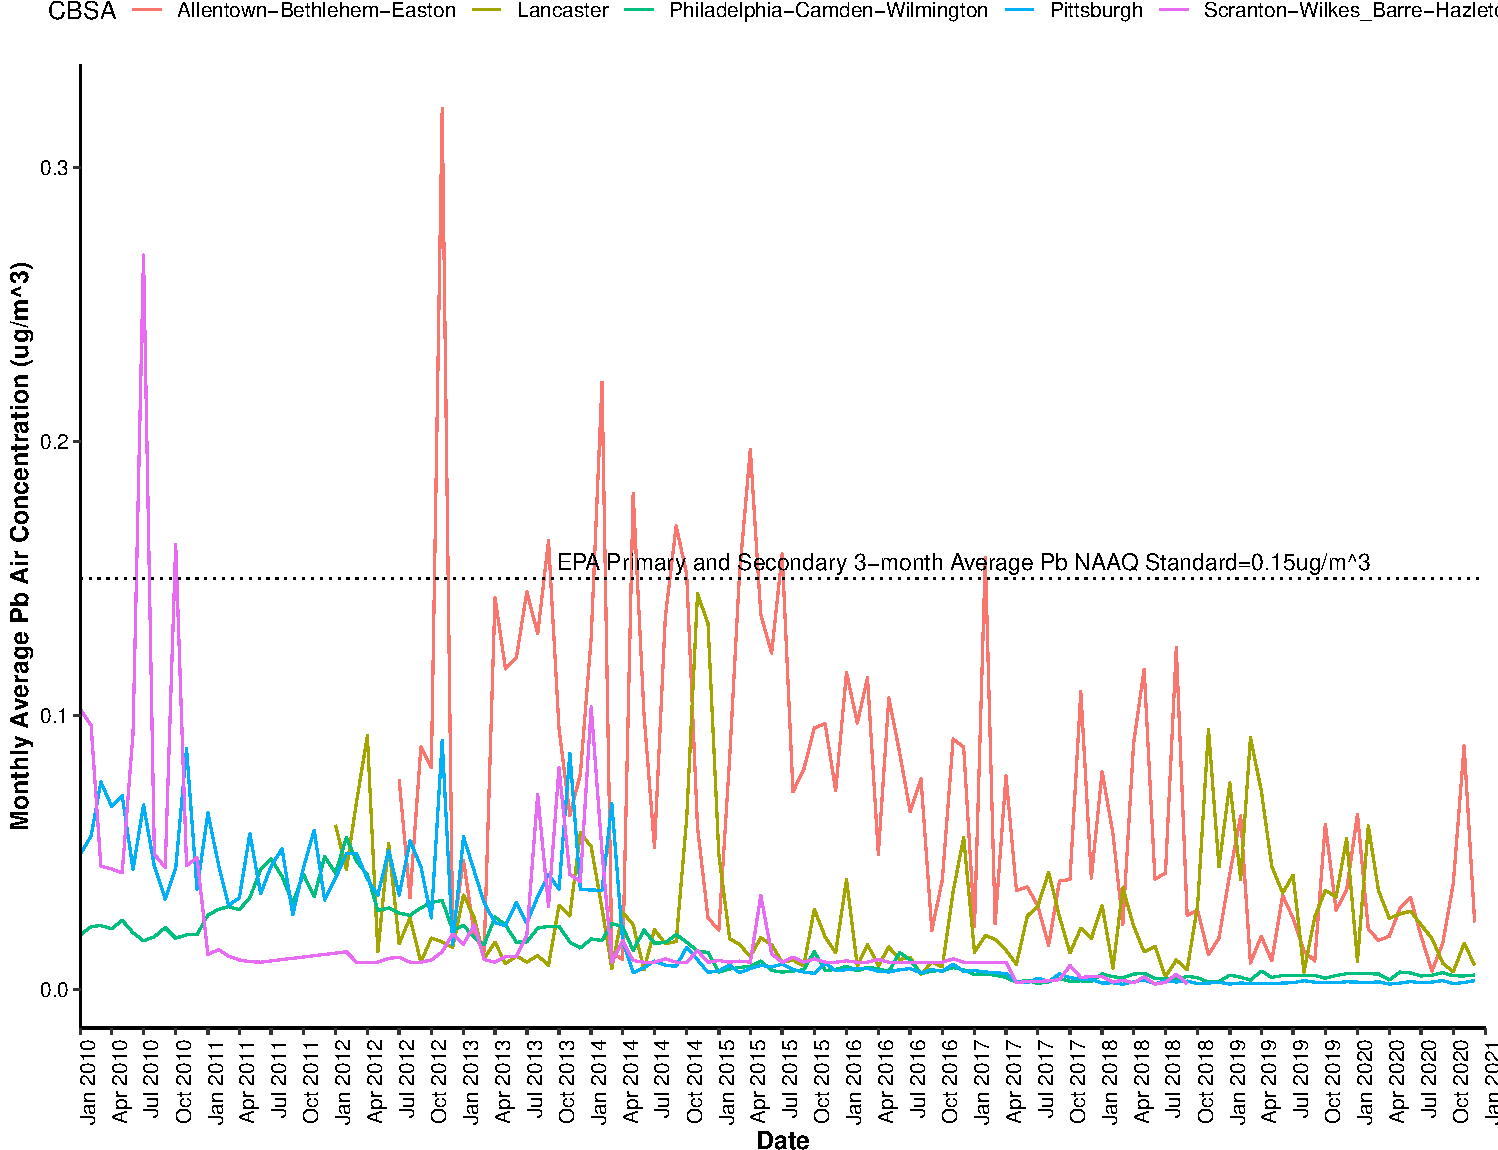
\includegraphics{Alcorn_Bao_Hermanson_ENV872_Project_files/figure-latex/time-series-visuals-1} \hfill{}

\caption{Monthly Average Pb Air Concentrations from 2010 to 2020 in PA Metro Areas}\label{fig:time-series-visuals}
\end{figure}

\begin{verbatim}
## [1] "Date"
\end{verbatim}

\begin{figure}

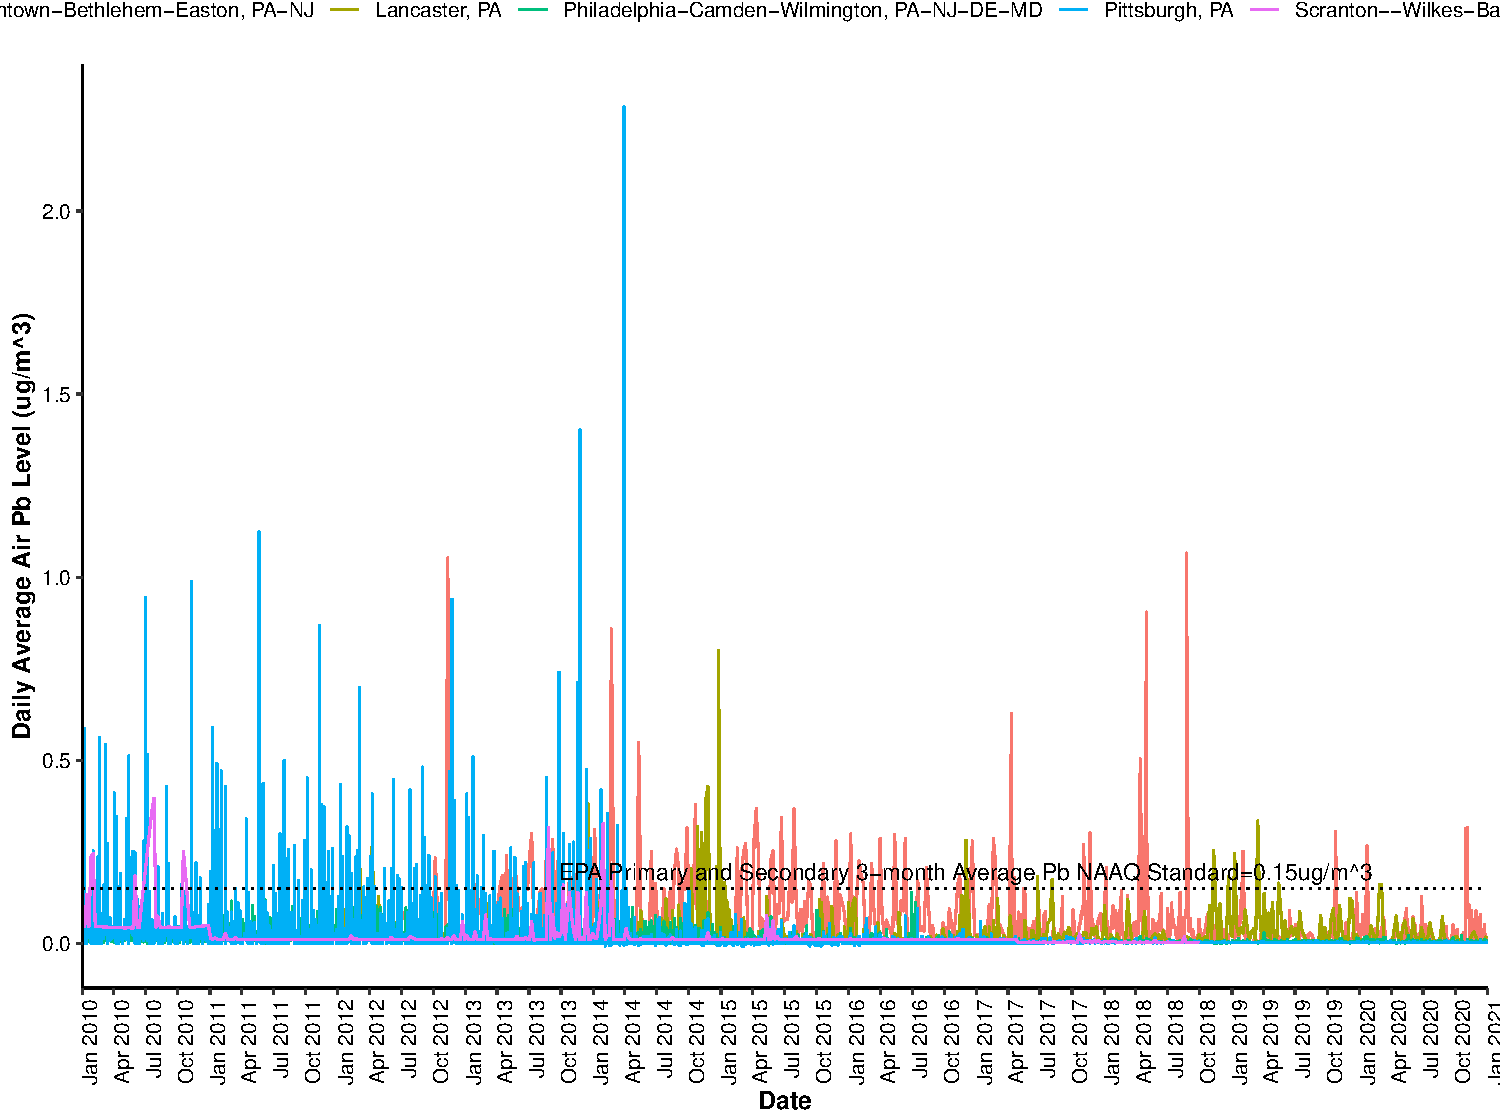
\includegraphics{Alcorn_Bao_Hermanson_ENV872_Project_files/figure-latex/linear-interp-visual-1} \hfill{}

\caption{Daily average air Pb levels from 2010 to 2020 in the five most populous metropolitan areas in PA}\label{fig:linear-interp-visual}
\end{figure}

\hypertarget{question-2-what-are-the-spatial-associations-between-air-lead-levels-and-socioeconomic-factors-ie.-income-and-poverty-across-counties-in-pennsylvania-1}{%
\subsection{Question 2: What are the spatial associations between air
lead levels and socioeconomic factors (ie. income and poverty) across
counties in
Pennsylvania?}\label{question-2-what-are-the-spatial-associations-between-air-lead-levels-and-socioeconomic-factors-ie.-income-and-poverty-across-counties-in-pennsylvania-1}}

The spatial analysis confirmed that mean lead concentration levels have
gone down from 2010 to 2020. The highest mean concentration levels for
2010 was .15 ug/m\^{}3 compared to .1 ug/m\^{}3 for 2015 and .03
ug/m\^{}3 for 2020. The graphs also showed where high lead
concentrations resided in the state of Pennsylvania. Counties that had
the highest concentrations were Lancaster, Berks, Lehigh, Beaver,
Allegheny, and Indiana. These are areas that have medium levels of
people below poverty and tend to have lower per capita income levels
compared with the rest of the state. When looking at the amount of
maximum lead concentration levels that were above the air quality
standard of .15 ug/m\^{}3, 2010 had 7 locations that exceeded this
limit. Berks and Beaver each had two areas with readings above .9
ug/m\^{}3. For 2015 and 2020, there were only three locations (for each
year) that exceeded the air quality standard limit. Beaver county had
zero areas during these years and Berks county reduced to only one
reading at approximately .24 ug/m\^{}3. This spatial analysis assists
with the time series analysis done in the section above. Moving forward,
doing an analysis at a smaller scale would provide improved results.
Future analysis could look at counties, such as Berks and Beaver, and
perform analysis at the zip code level.

\begin{verbatim}
## `summarise()` has grouped output by 'COUNTY', 'SITE_LATITUDE'. You can override using the `.groups` argument.
\end{verbatim}

\begin{verbatim}
## [1] 0.02118966 0.17580357
\end{verbatim}

\begin{verbatim}
## Reading layer `cb_2018_us_county_20m' from data source `/Users/mothership/Desktop/EDA_21/Alcorn_Bao_Hermanson_ENV_872_EDA_FinalProject/Data/Spatial/cb_2018_us_county_20m.shp' using driver `ESRI Shapefile'
## Simple feature collection with 3220 features and 9 fields
## Geometry type: MULTIPOLYGON
## Dimension:     XY
## Bounding box:  xmin: -179.1743 ymin: 17.91377 xmax: 179.7739 ymax: 71.35256
## Geodetic CRS:  NAD83
\end{verbatim}

\begin{verbatim}
## [1] 15691.33 40670.86
\end{verbatim}

\begin{figure}

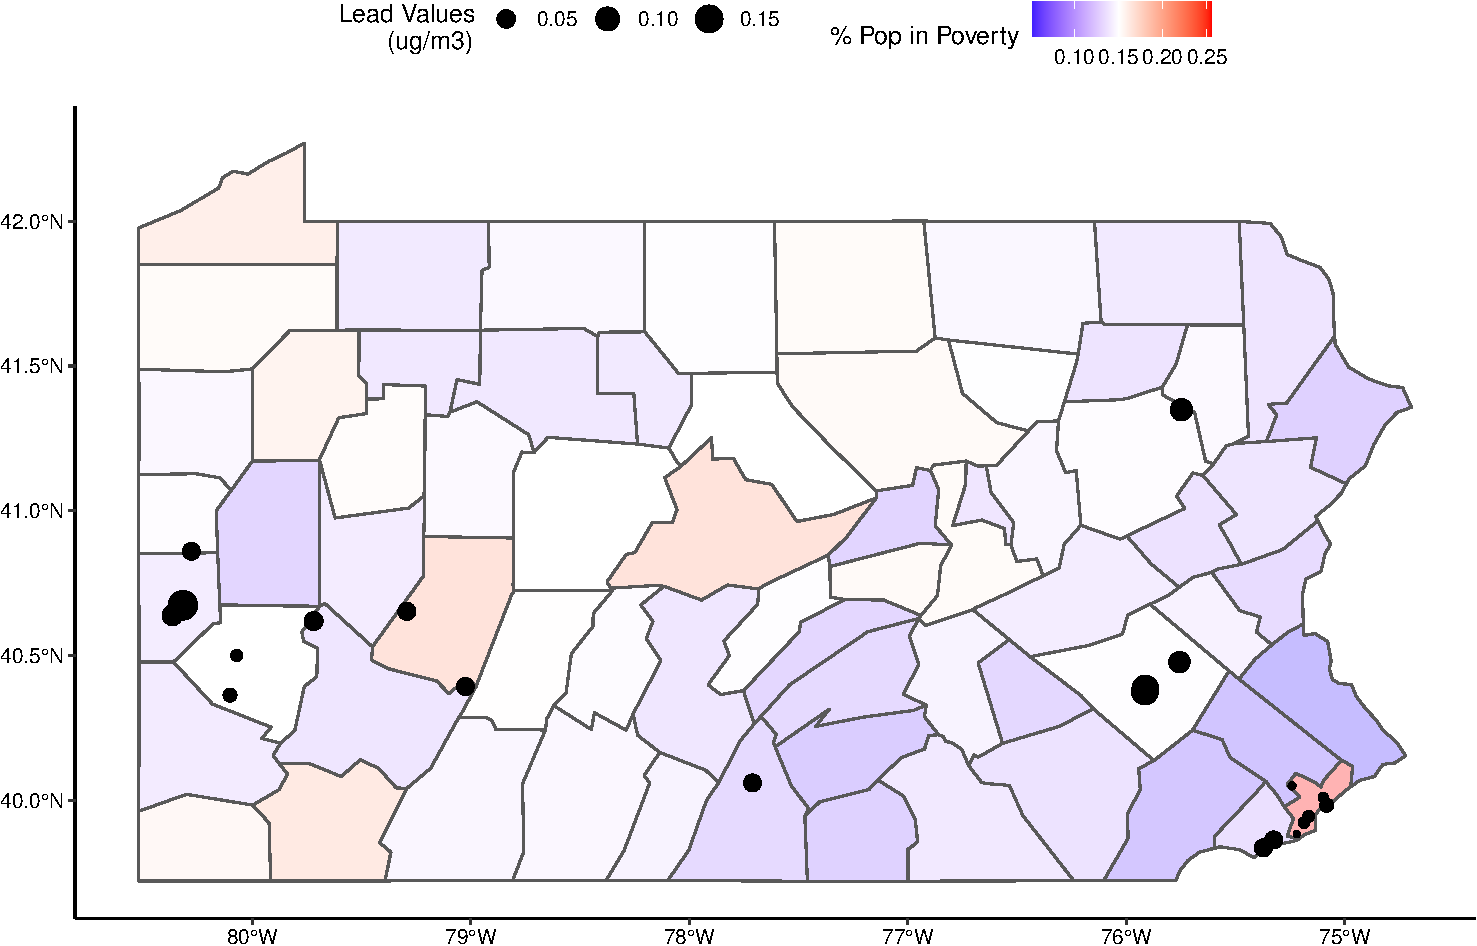
\includegraphics{Alcorn_Bao_Hermanson_ENV872_Project_files/figure-latex/spatial-analysis 2010-1} \hfill{}

\caption{2010 Mean Lead Levels Across Pennsylvania}\label{fig:spatial-analysis 2010}
\end{figure}

\begin{figure}

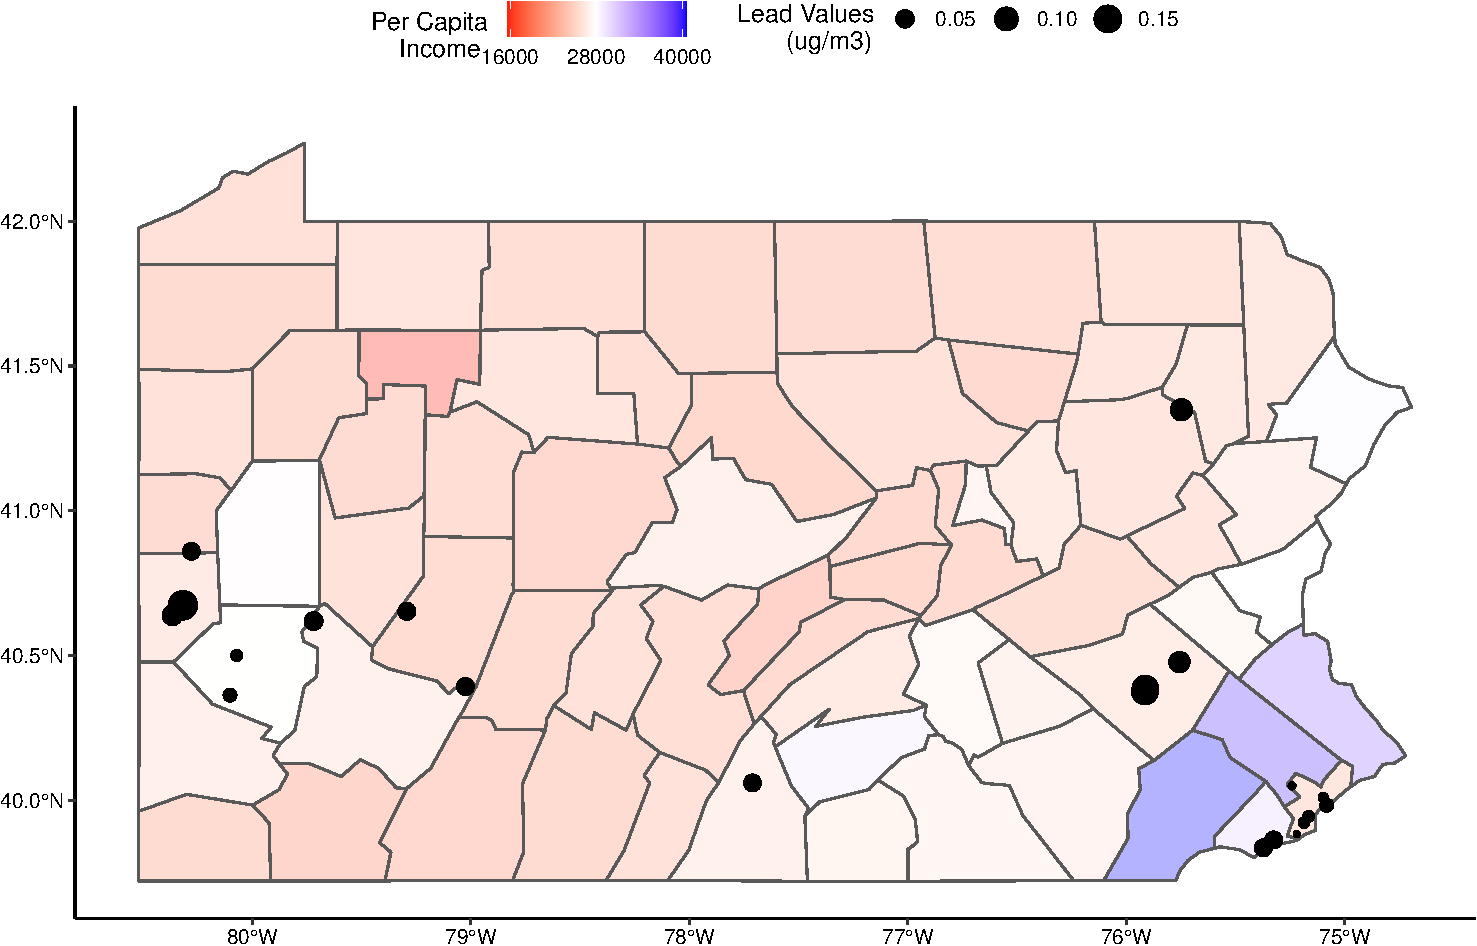
\includegraphics{Alcorn_Bao_Hermanson_ENV872_Project_files/figure-latex/spatial analysis 2010.2-1} \hfill{}

\caption{2010 Mean Lead Levels Across Pennsylvania}\label{fig:spatial analysis 2010.2}
\end{figure}

\begin{figure}

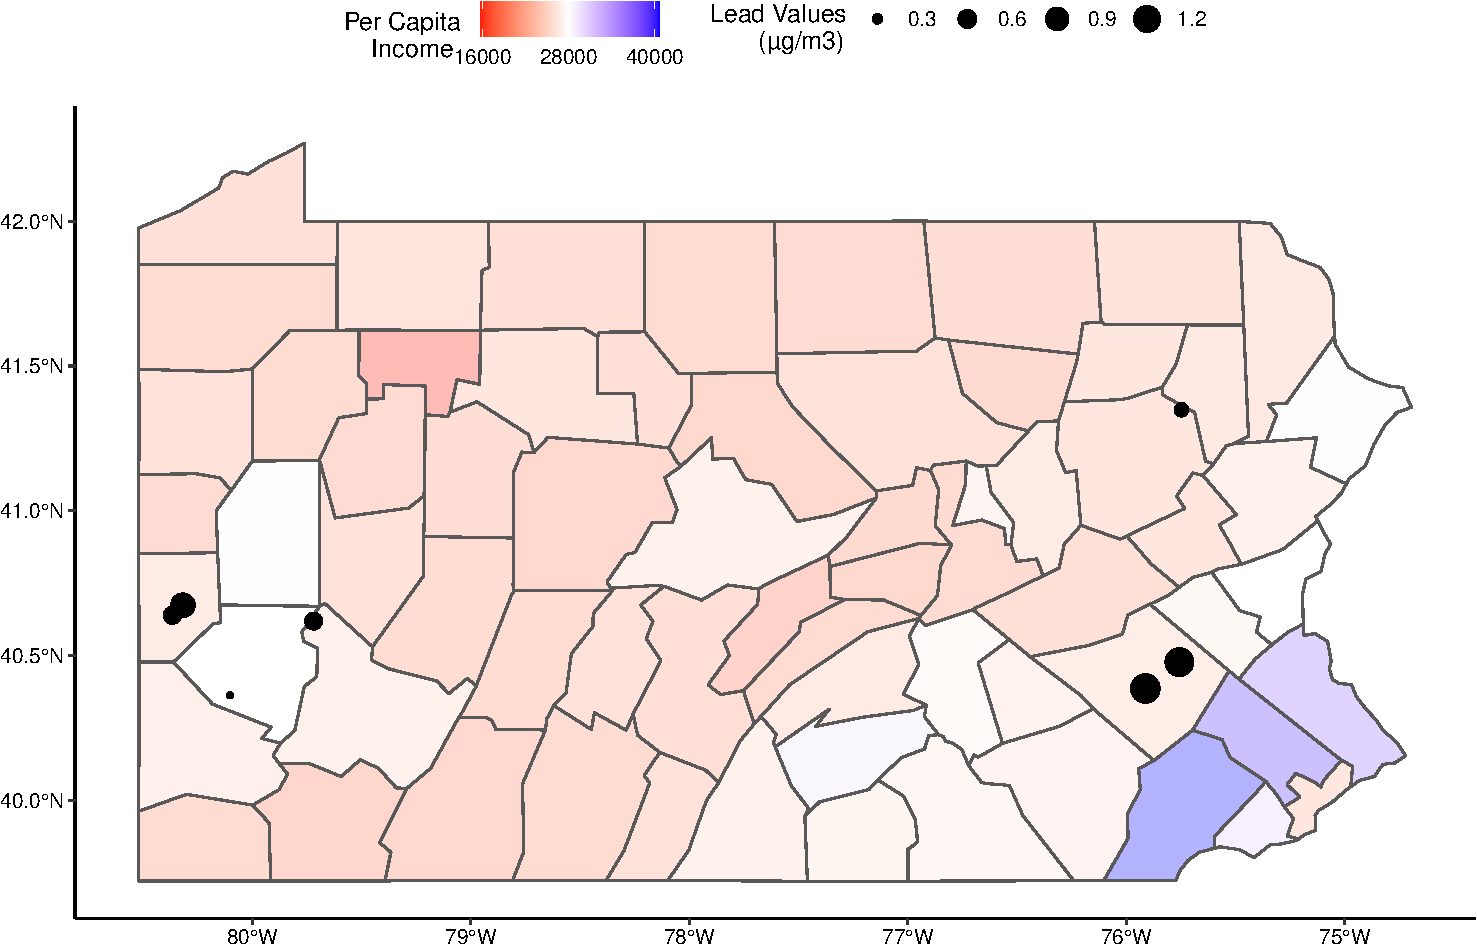
\includegraphics{Alcorn_Bao_Hermanson_ENV872_Project_files/figure-latex/spatial-analysis 2010.3-1} \hfill{}

\caption{2010 Max Lead Levels over .15 (µg/m3)}\label{fig:spatial-analysis 2010.3}
\end{figure}

\begin{verbatim}
## `summarise()` has grouped output by 'COUNTY', 'SITE_LATITUDE'. You can override using the `.groups` argument.
\end{verbatim}

\begin{verbatim}
## [1] 0.02118966 0.17580357
\end{verbatim}

\begin{figure}

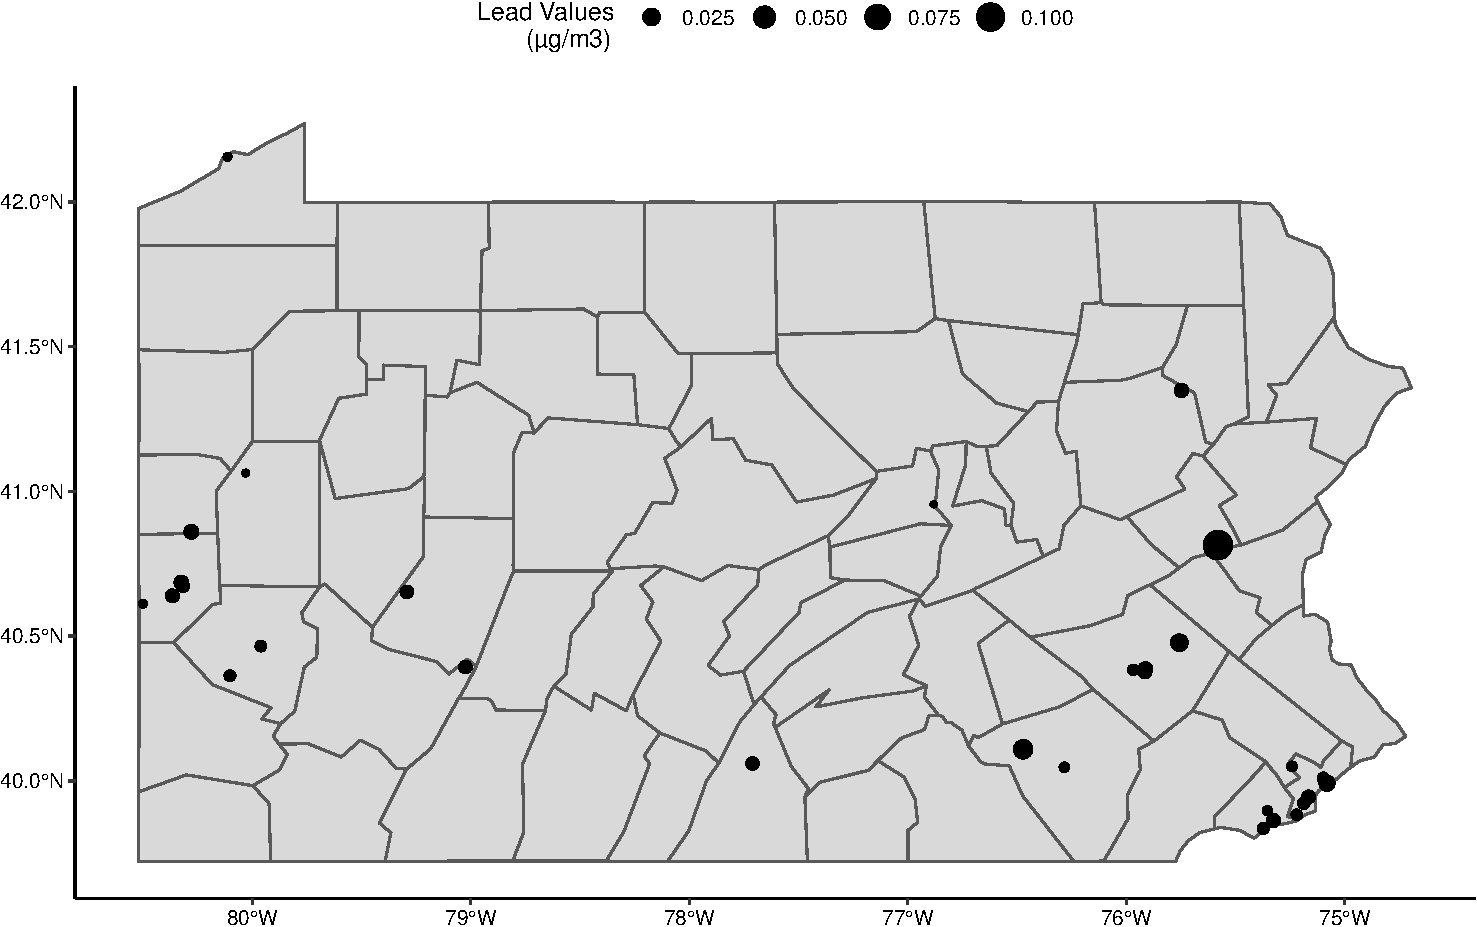
\includegraphics{Alcorn_Bao_Hermanson_ENV872_Project_files/figure-latex/spatial analysis 2015.4-1} \hfill{}

\caption{2015 Mean Lead Levels Across Pennsylvania}\label{fig:spatial analysis 2015.4}
\end{figure}

\begin{figure}
\centering
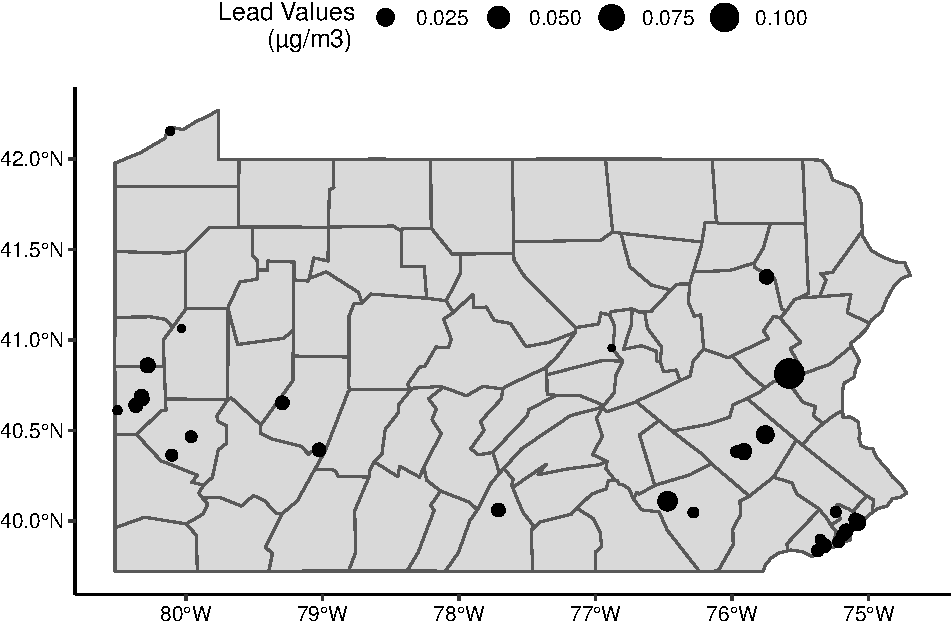
\includegraphics{Alcorn_Bao_Hermanson_ENV872_Project_files/figure-latex/spatial analysis 2015.5-1.pdf}
\caption{2015 Mean Lead Levels Across Pennsylvania}
\end{figure}

\begin{figure}
\centering
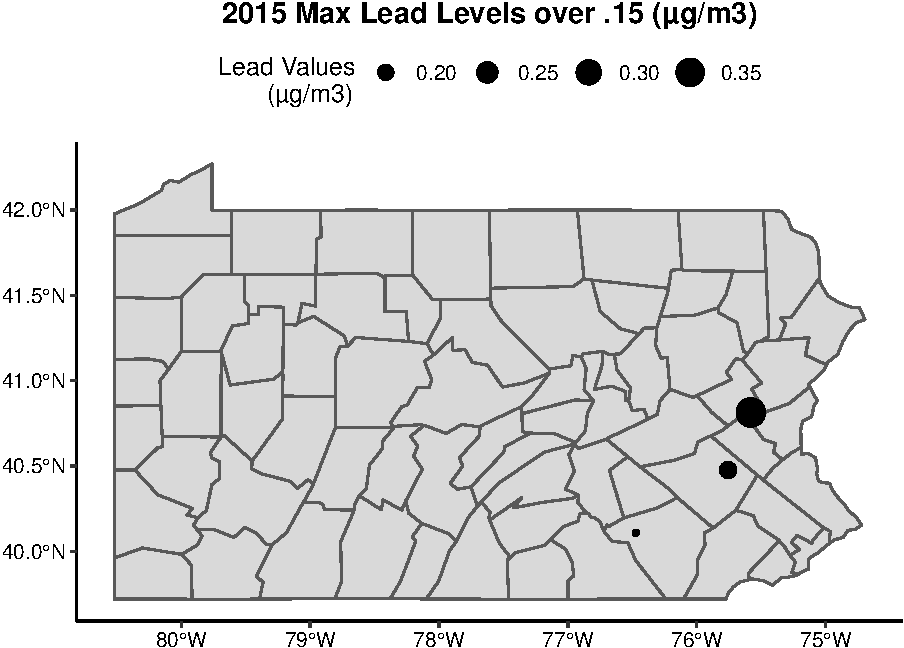
\includegraphics{Alcorn_Bao_Hermanson_ENV872_Project_files/figure-latex/spatial analysis 2015.6-1.pdf}
\caption{2015 Max Lead Levels over .15 (µg/m3)}
\end{figure}

\begin{verbatim}
## `summarise()` has grouped output by 'COUNTY', 'SITE_LATITUDE'. You can override using the `.groups` argument.
\end{verbatim}

\begin{figure}

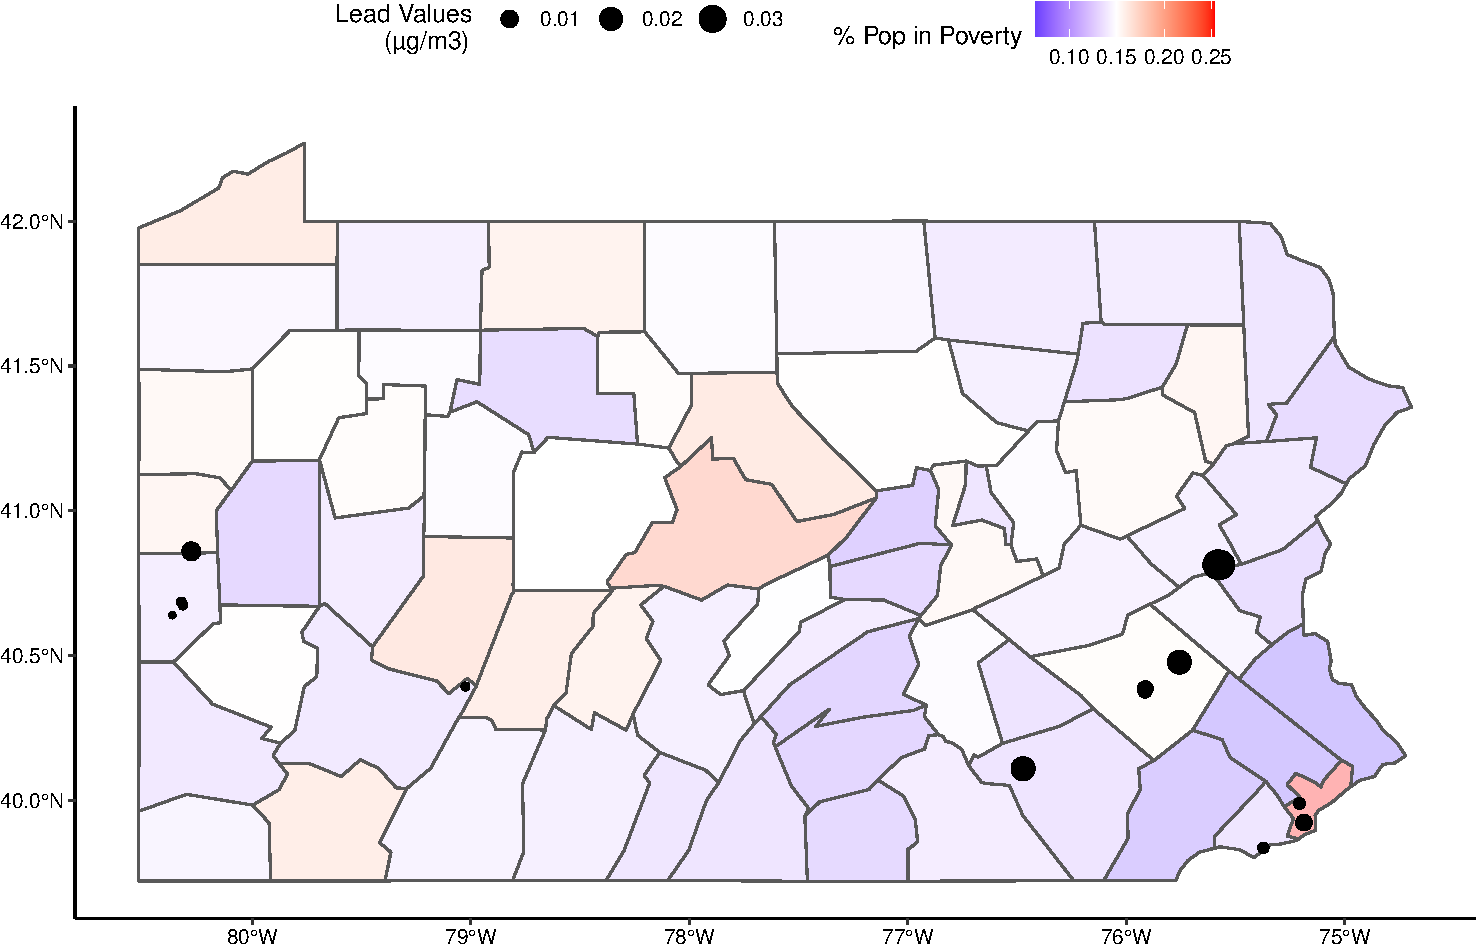
\includegraphics{Alcorn_Bao_Hermanson_ENV872_Project_files/figure-latex/spatial analysis 2020.1-1} \hfill{}

\caption{2020 Mean Lead Levels Across Pennsylvania}\label{fig:spatial analysis 2020.1}
\end{figure}

\begin{figure}

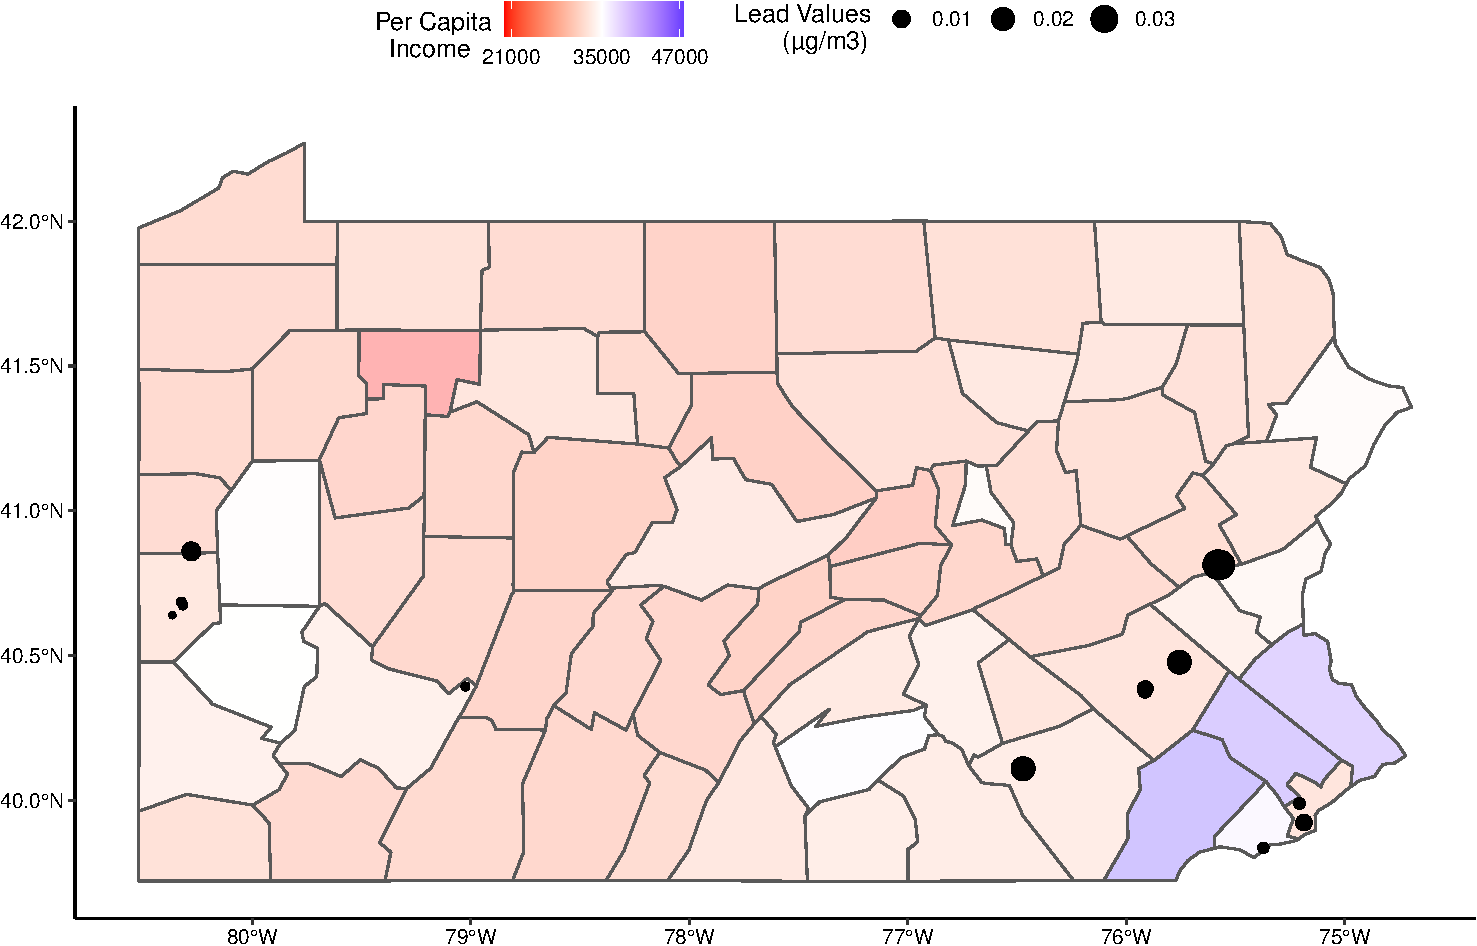
\includegraphics{Alcorn_Bao_Hermanson_ENV872_Project_files/figure-latex/spatial analysis 2020.2-1} \hfill{}

\caption{2020 Mean Lead Levels Across Pennsylvania}\label{fig:spatial analysis 2020.2}
\end{figure}

\begin{figure}

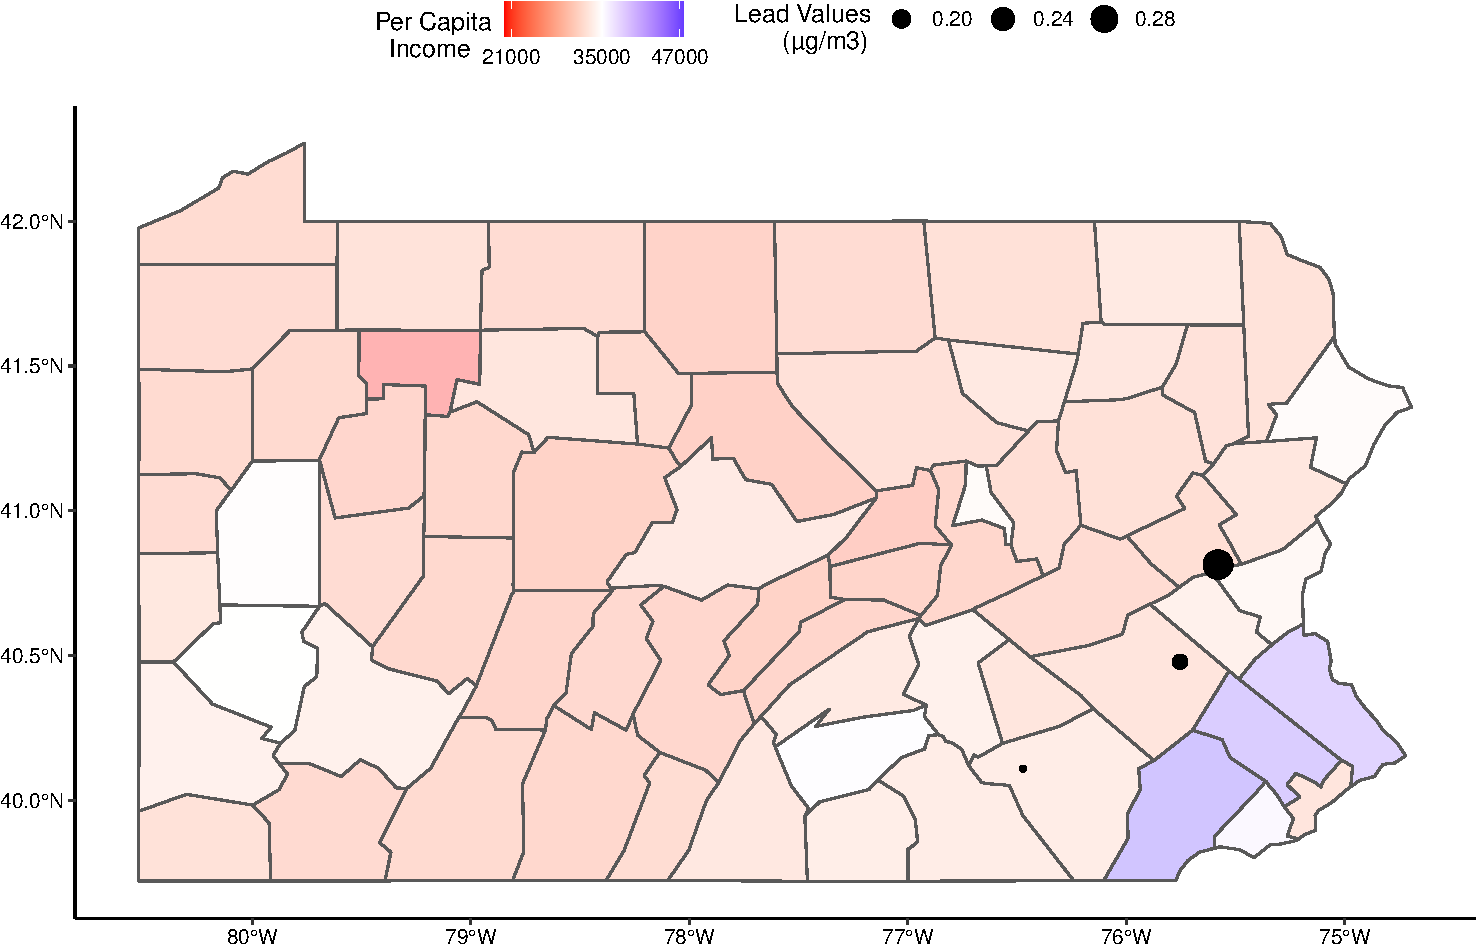
\includegraphics{Alcorn_Bao_Hermanson_ENV872_Project_files/figure-latex/spatial analysis 2020.3-1} \hfill{}

\caption{2020 Max Lead Levels over .15 (µg/m3)}\label{fig:spatial analysis 2020.3}
\end{figure}

\hypertarget{final-model-model-9}{%
\subsubsection{Final Model (Model 9)}\label{final-model-model-9}}

\hypertarget{blood-lead-beta1-x-log_metal-beta2-x-log_incinerate-beta4-x-meanpercapincome-beta5-x-pov2}{%
\paragraph{Blood lead = (beta1 x log\_metal) + (beta2 x log\_incinerate)
+ (beta4 x meanPerCapIncome) + (beta5 x
POV\$\^{}\$2)}\label{blood-lead-beta1-x-log_metal-beta2-x-log_incinerate-beta4-x-meanpercapincome-beta5-x-pov2}}

This model is statistically insignificant overall, with an f-statistics
p-value (0.29) being far greater than 0.05. The coefficient of meanPCI
(mean per-capita income) was statistically significant (p \textless{}
0.05), and can be interpreted as every decrease in income by 2,877
dollars is correlated with a 1\% increase in blood-lead levels in
children.

The low significance of this model is not surprising, given the
limitations of the data. The number of metal/incinerator plants may not
necessarily reflect the quantity of particulate lead being emitted,
which likely varies greatly between plants. If data were able to be
obtained about how much smoke/lead-particulate matter is being emitted
per plant, then that would have been more useful. The same applies to
airports; it is likely that the quantity of airports does not matter so
much as the number of flights and size of planes cycling through each
airport; were FAA data on these parameters available, they would have
been carried out. This is ultimately why the airport data was omitted
from the final model.

Quantity of plants/airports would have been more useful if the
geographic units used in this model were smaller -- county-level data
was the smallest data we could work with, given the reported blood lead
levels reported by the CDC were at a county level. Another geographical
consideration is that lead-emissions from the studied sources may not
affect their respective counties and instead disperse to other counties.

Of further concern with the metal processing data was that the range of
metal-processing plants was low across counties (max number of plants
was 12, min 0), with the mean being 1.72 plants/county. Such skewness of
the mean may not be appropriate for an OLS regression.

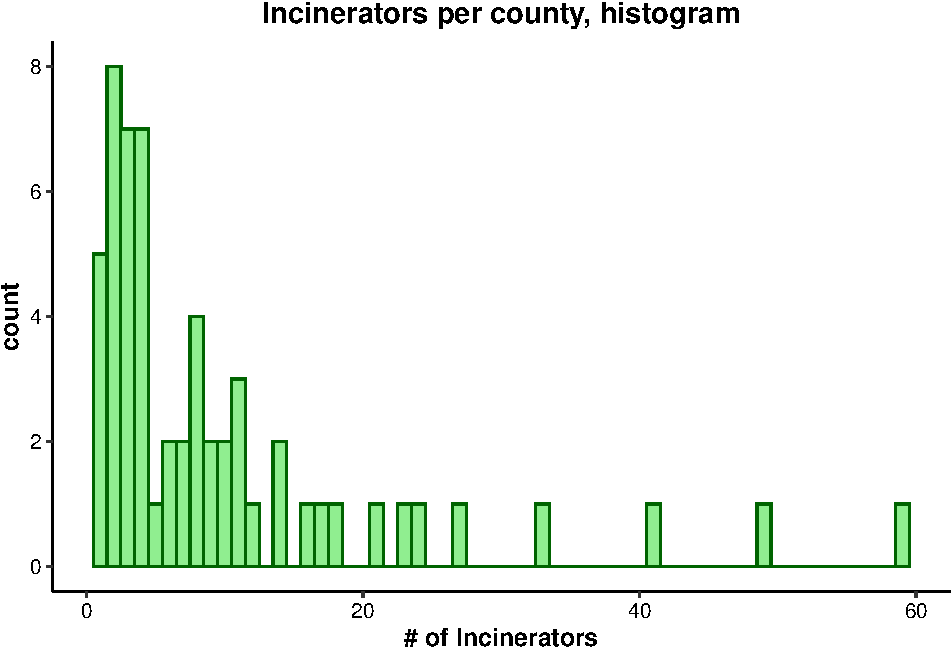
\includegraphics{Alcorn_Bao_Hermanson_ENV872_Project_files/figure-latex/setuping section-1.pdf}
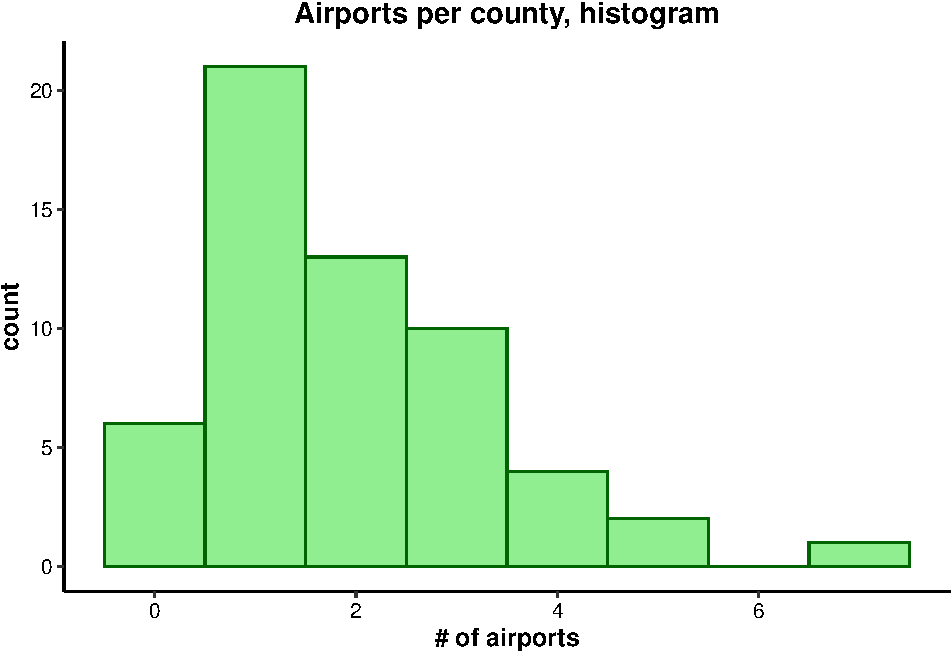
\includegraphics{Alcorn_Bao_Hermanson_ENV872_Project_files/figure-latex/setuping section-2.pdf}
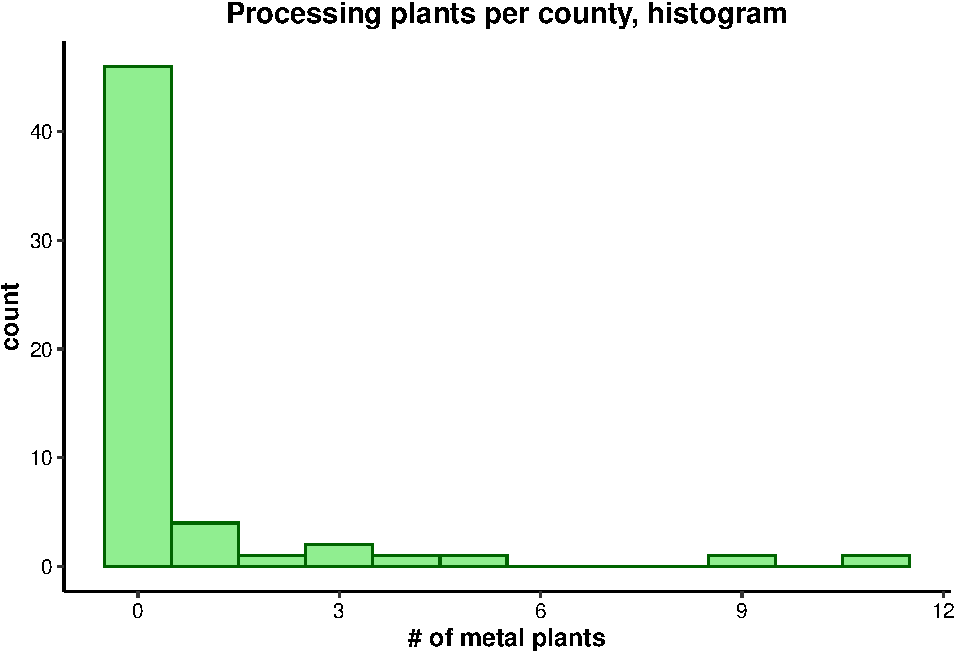
\includegraphics{Alcorn_Bao_Hermanson_ENV872_Project_files/figure-latex/setuping section-3.pdf}

\begin{verbatim}
## Rows: 1
## Columns: 6
## $ Length  <int> 57
## $ Mean    <dbl> 0.7192982
## $ Median  <dbl> 0
## $ Std_Dev <dbl> 2.068077
## $ Minimum <dbl> 0
## $ Maximum <dbl> 11
\end{verbatim}

\begin{verbatim}
## Rows: 1
## Columns: 6
## $ Length  <int> 57
## $ Mean    <dbl> 10.03509
## $ Median  <int> 6
## $ Std_Dev <dbl> 11.93728
## $ Minimum <int> 1
## $ Maximum <int> 59
\end{verbatim}

\begin{verbatim}
## Rows: 1
## Columns: 6
## $ Length  <int> 57
## $ Mean    <dbl> 1.929825
## $ Median  <dbl> 2
## $ Std_Dev <dbl> 1.425027
## $ Minimum <dbl> 0
## $ Maximum <dbl> 7
\end{verbatim}

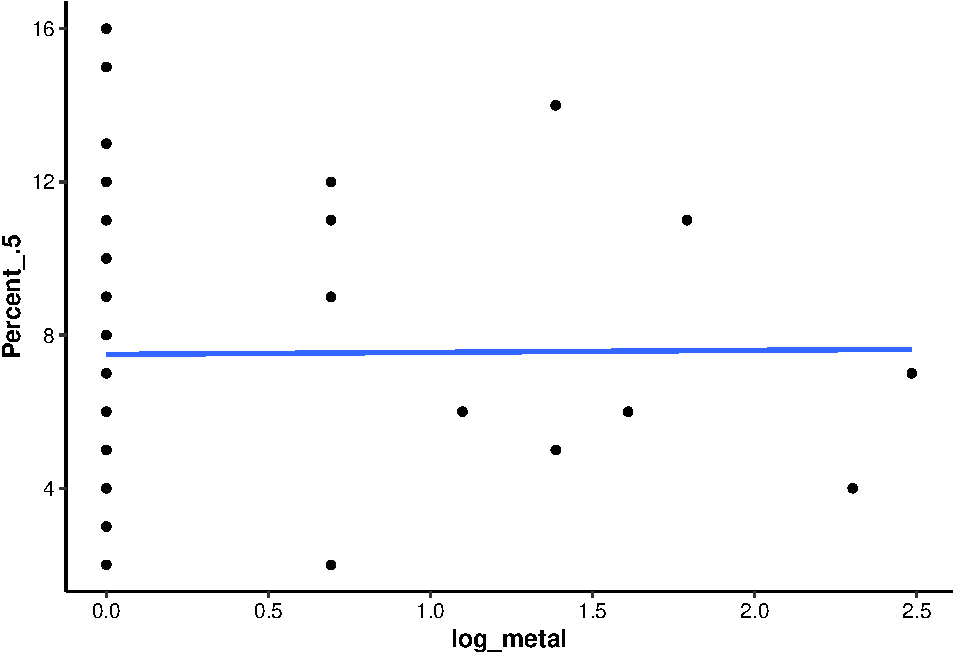
\includegraphics{Alcorn_Bao_Hermanson_ENV872_Project_files/figure-latex/linear plotssss -1.pdf}
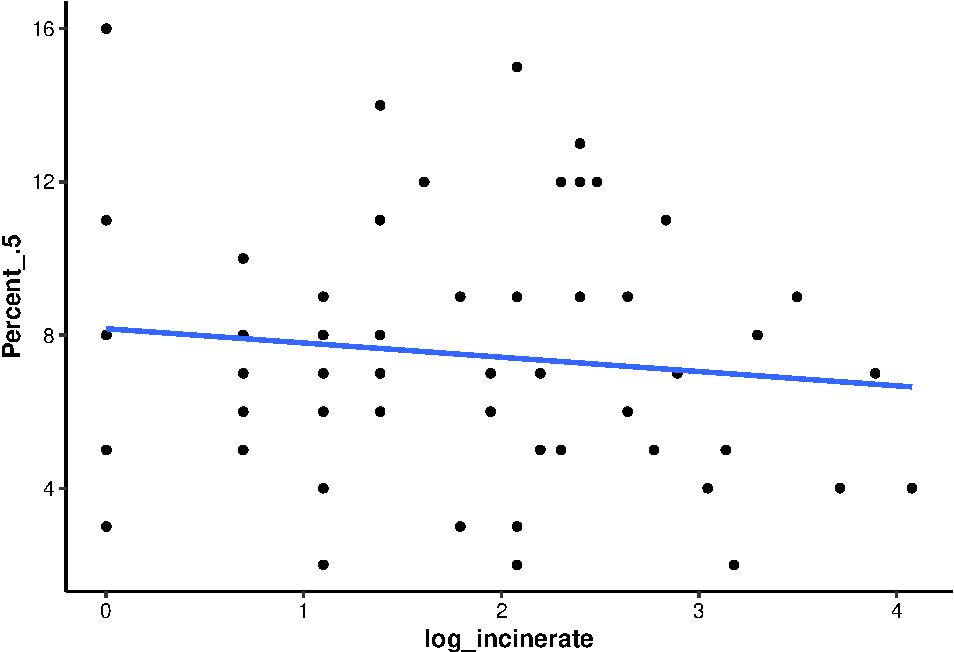
\includegraphics{Alcorn_Bao_Hermanson_ENV872_Project_files/figure-latex/linear plotssss -2.pdf}
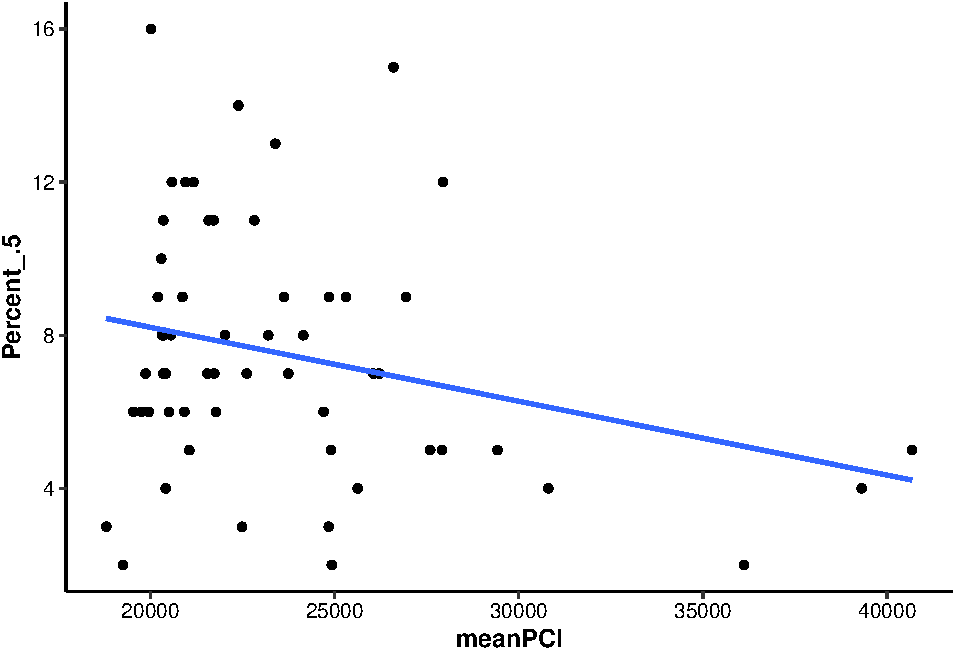
\includegraphics{Alcorn_Bao_Hermanson_ENV872_Project_files/figure-latex/linear plotssss -3.pdf}
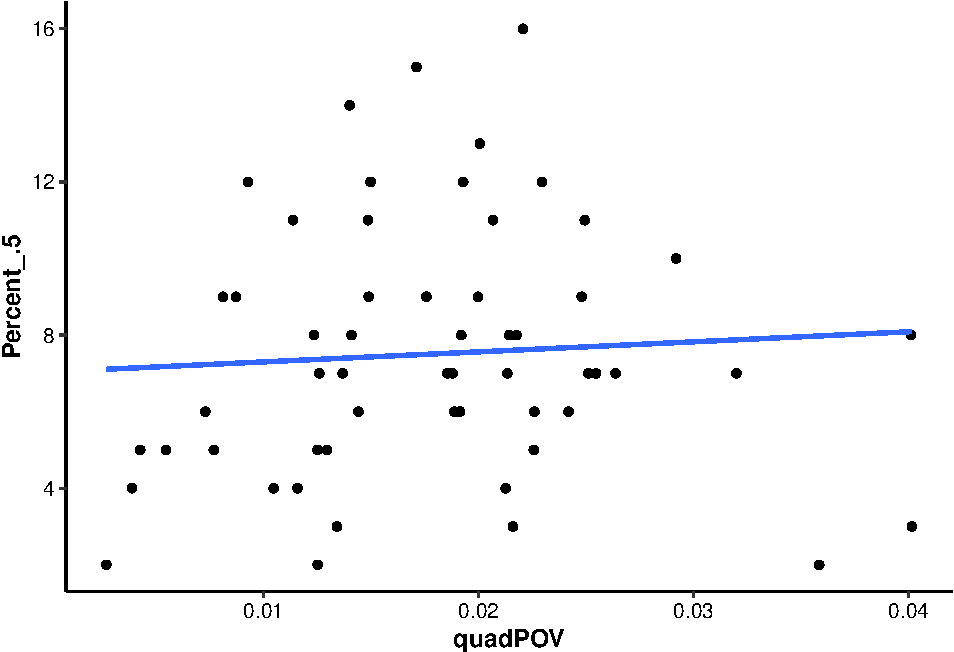
\includegraphics{Alcorn_Bao_Hermanson_ENV872_Project_files/figure-latex/linear plotssss -4.pdf}
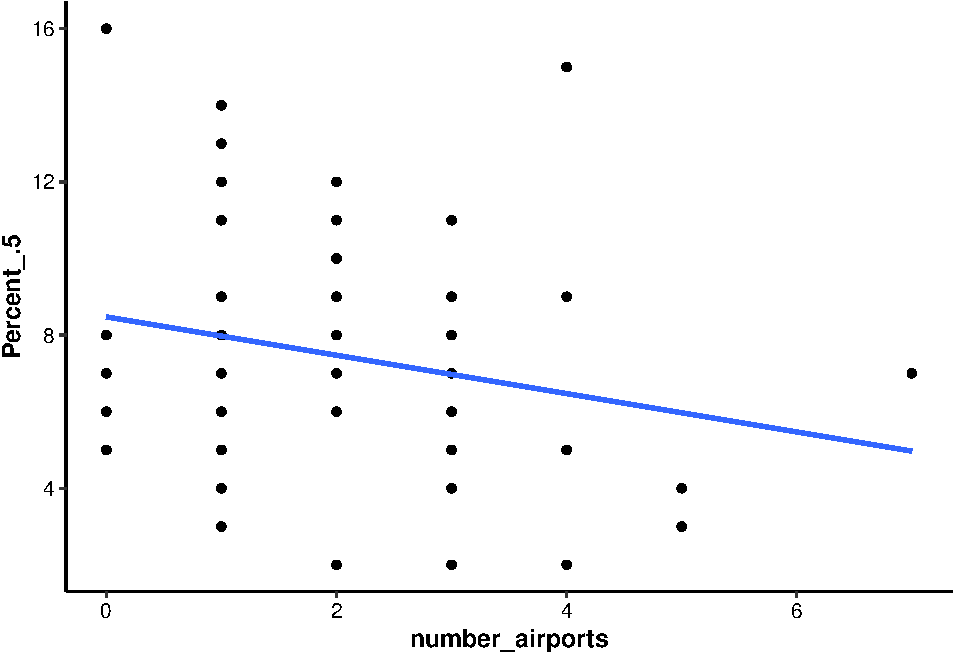
\includegraphics{Alcorn_Bao_Hermanson_ENV872_Project_files/figure-latex/linear plotssss -5.pdf}

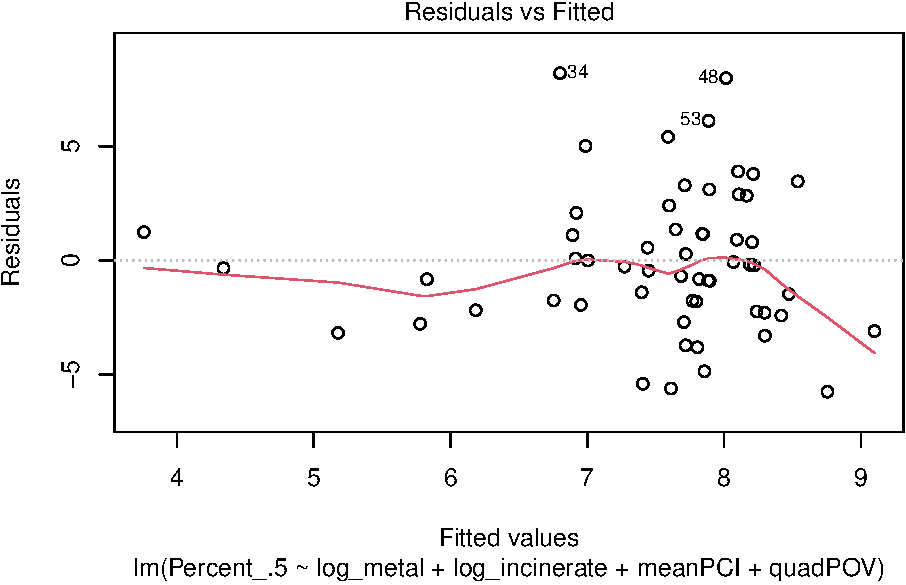
\includegraphics{Alcorn_Bao_Hermanson_ENV872_Project_files/figure-latex/analysis tools2-1.pdf}
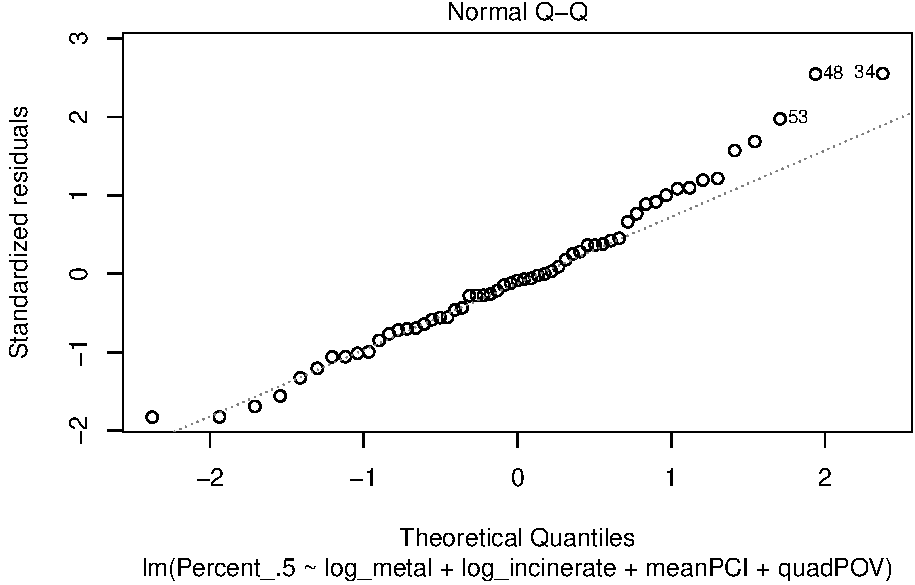
\includegraphics{Alcorn_Bao_Hermanson_ENV872_Project_files/figure-latex/analysis tools2-2.pdf}
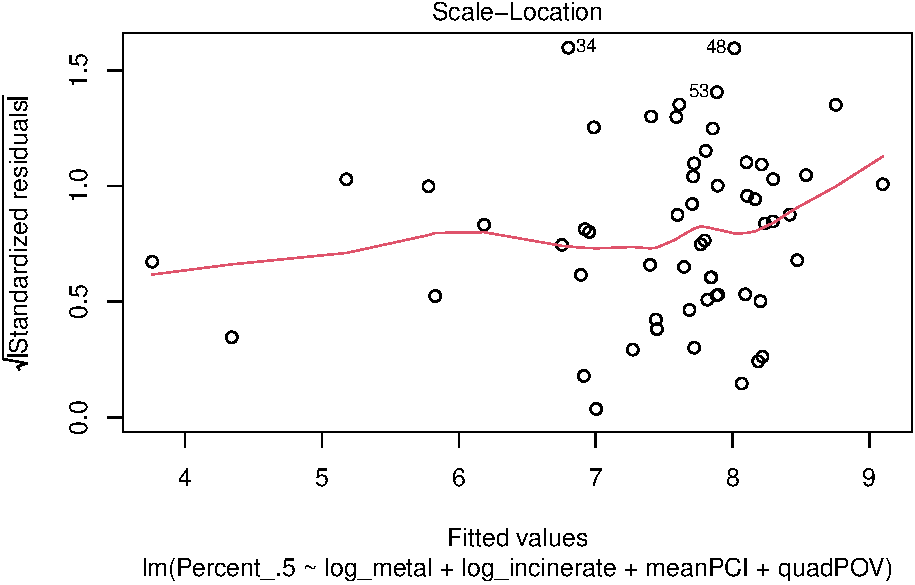
\includegraphics{Alcorn_Bao_Hermanson_ENV872_Project_files/figure-latex/analysis tools2-3.pdf}
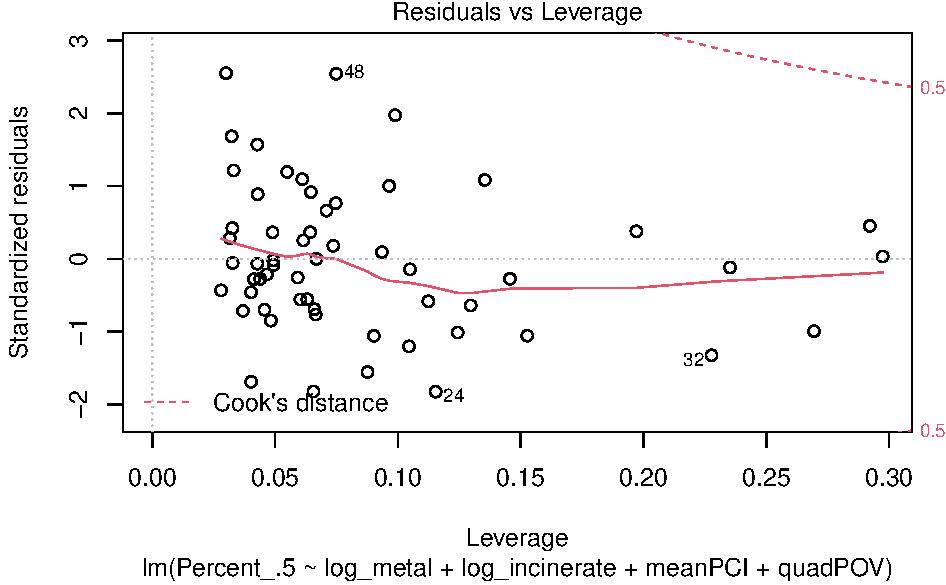
\includegraphics{Alcorn_Bao_Hermanson_ENV872_Project_files/figure-latex/analysis tools2-4.pdf}

\begin{figure}

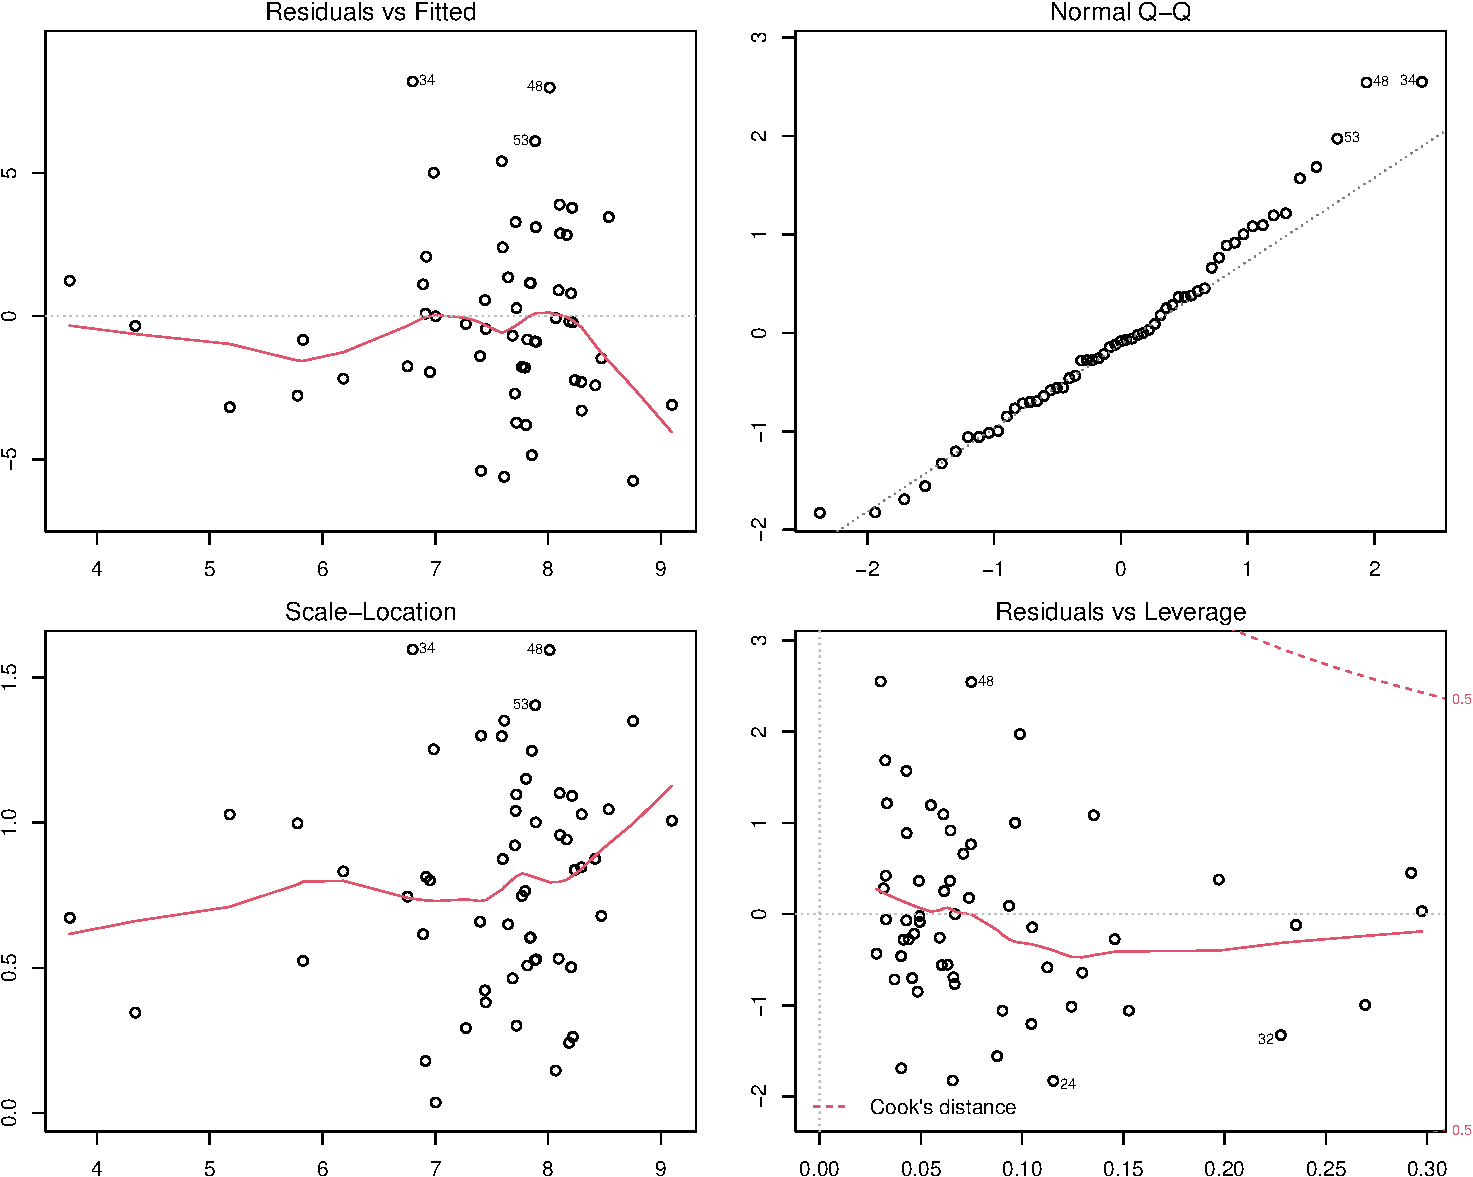
\includegraphics{Alcorn_Bao_Hermanson_ENV872_Project_files/figure-latex/analyis final-1} \hfill{}

\caption{Model Assumption Plots}\label{fig:analyis final}
\end{figure}

\begin{verbatim}
## 
## Call:
## lm(formula = Percent_.5 ~ log_metal + log_incinerate + meanPCI + 
##     quadPOV, data = i_a_m_b_join)
## 
## Residuals:
##     Min      1Q  Median      3Q     Max 
## -5.7545 -2.1846 -0.2716  1.3546  8.2000 
## 
## Coefficients:
##                  Estimate Std. Error t value Pr(>|t|)    
## (Intercept)     1.519e+01  3.865e+00   3.929 0.000253 ***
## log_metal      -1.463e-01  7.386e-01  -0.198 0.843749    
## log_incinerate  1.749e-01  4.964e-01   0.352 0.725962    
## meanPCI        -2.877e-04  1.403e-04  -2.051 0.045363 *  
## quadPOV        -6.406e+01  6.798e+01  -0.942 0.350397    
## ---
## Signif. codes:  0 '***' 0.001 '**' 0.01 '*' 0.05 '.' 0.1 ' ' 1
## 
## Residual standard error: 3.264 on 52 degrees of freedom
## Multiple R-squared:  0.08933,    Adjusted R-squared:  0.01928 
## F-statistic: 1.275 on 4 and 52 DF,  p-value: 0.2917
\end{verbatim}

\begin{verbatim}
## [1] 303.3744
\end{verbatim}

\begin{verbatim}
##      log_metal log_incinerate        meanPCI        quadPOV 
##       1.044164       1.422348       2.158539       1.639418
\end{verbatim}

\begin{verbatim}
## number_metal_plants number_incinerators     number_airports             meanPCI 
##            1.053063            2.118427            1.871259            2.954335 
##             meanPOV 
##            2.189966
\end{verbatim}

\newpage

\hypertarget{summary-and-conclusions}{%
\section{Summary and Conclusions}\label{summary-and-conclusions}}

We found that four of the five most populous metropolitan areas
Philadelphia-Camden-Wilmington, PA-NJ-DE-MD (2010-2020), Pittsburgh, PA
(2010-2020), Allentown-Bethlehem-Easton, PA-NJ (2012-2020), and
Scranton--Wilkes-Barre--Hazleton, PA (2010-2018) in Pennsylvania had
downward monotonic trends for daily and monthly mean air lead
concentrations (p\textless0.05). The Lancaster, PA metropolitan area did
not show a monotonic downward trend for air lead levels, which may be
attributed to other factors not explored in this study such as
industrial emissions between 2012 and 2020. It is important to note that
the downward trend for the other four metropolitan areas may be
attributed to the banning of lead in paints in 1978, the banning of lead
in vehicle fuels in 1996, the waning of lead-smelting industry, or other
factors such as lead abatement programs from 2010 to 2020 in
Pennsylvania into the twenty-first century (Schwarz et al., 2012).
Future studies may look at conducting multiple linear regression to
assess air lead levels in association with remediation measures to
reduce air lead exposure or other factors such as climate factors like
temperature and wind speed, which may influence quantity of lead in
ambient air (Kinney, 2018). Obtaining census-block specific data and air
emissions data will enable stronger multilinear regression in future
models.

\newpage

\hypertarget{references}{%
\section{References}\label{references}}

Ab Latif Wani, A. A., \& Usmani, J. A. (2015). Lead toxicity: a review.
Interdisciplinary toxicology, 8(2), 55. doi: 10.1515/intox-2015-0009

About Air Data Reports. (2021). United States Environmental Protection
Agency. Retrieved from
\href{https://www.epa.gov/outdoor-air-quality-data/about-air-data-reports}{link}

American Lung Association (2021). Most Polluted Cities. Retrieved from
\href{https://www.lung.org/research/sota/city-rankings/most-polluted-cities}{link}

CDC Social Vulnerability Index Data {[}internet database{]} available
via
\href{https://www.atsdr.cdc.gov/placeandhealth/svi/data_documentation_download.html}{link}

Kinney, P. L. (2018). Interactions of climate change, air pollution, and
human health. Current environmental health reports, 5(1), 179-186.
\href{https://doi.org/10.1007/s40572-018-0188-x}{link}

O'Shea, M. J., Vann, D. R., Hwang, W. T., \& Gieré, R. (2020). A
mineralogical and chemical investigation of road dust in Philadelphia,
PA, USA. Environmental Science and Pollution Research, 1-20.
\href{https://doi.org/10.1007/s11356-019-06746-y}{link}

PA Department of Health (2014). 2014 Childhood Lead Surveillance Annual
Report. Retrieved from
\href{https://www.health.pa.gov/topics/Documents/Environmental\%20Health/2014\%20Lead\%20Surveillance\%20Annual\%20Report.pdf}{link}

Pizzol, M., Thomsen, M., \& Andersen, M. S. (2010). Long-term human
exposure to lead from different media and intake pathways. Science of
the total environment, 408(22), 5478-5488.
\href{https://doi.org/10.1016/j.scitotenv.2010.07.077}{link}

Schwarz, K., Pickett, S. T., Lathrop, R. G., Weathers, K. C., Pouyat, R.
V., \& Cadenasso, M. L. (2012). The effects of the urban built
environment on the spatial distribution of lead in residential soils.
Environmental pollution, 163, 32-39.
\href{https://doi.org/10.1016/j.envpol.2011.12.003}{link}

Stevens, S. K. (1955). A Century of Industry in Pennsylvania.
Pennsylvania History: A Journal of Mid-Atlantic Studies, 22(1), 49-68.

United Health Foundation. (2019). America's Health Rankings. Retrieved
from
\href{https://assets.americashealthrankings.org/app/uploads/ahr_2019annualreport.pdf}{link}

US Census Bureau. (2019). Metropolitan and Micropolitan Statistical Area
Population Estimates and Estimated Components of Change: April 1, 2010
to July 1, 2019 (CBSA-EST2019-alldata). Retrieved from
\href{https://www.census.gov/data/tables/time-series/demo/popest/2010s-total-metro-and-micro-statistical-areas.html\#par_textimage}{link}

US Census Bureau. (2020a). CBSA-EST2019-alldata: Annual Resident
Population Estimates and Estimated Components of Resident Population
Change for Metropolitan and Micropolitan Statistical Areas and Their
Geographic Components: April 1, 2010 to July 1, 2019
\href{https://www2.census.gov/programs-surveys/popest/technical-documentation/file-layouts/2010-2019/cbsa-est2019-alldata.pdf}{link}

US Census Bureau (2020b). METHODOLOGY FOR THE UNITED STATES POPULATION
ESTIMATES: VINTAGE 2019 Nation, States, Counties, and Puerto Rico --
April 1, 2010 to July 1, 2019. Retrieved from
\href{https://www2.census.gov/programs-surveys/popest/technical-documentation/methodology/2010-2019/natstcopr-methv2.pdf}{link}

US Environmental Protection Agency. Air Quality System Data Mart
{[}internet database{]} available via
\href{https://www.epa.gov/airdata.\%20Accessed\%20April\%2005,\%202021.}{link}

US EPA. (2021a). Basic Information about Lead Air Pollution. Lead Air
Pollution. Retrieved from
\href{https://www.epa.gov/lead-air-pollution/basic-information-about-lead-air-pollution\#:~:text=At\%20the\%20national\%20level\%2C\%20major,usually\%20found\%20near\%20lead\%20smelters.}{link}

US EPA. (2021b). Timeline of Lead (Pb) National Ambient Air Quality
Standards (NAAQS) Retrieved from
\href{https://www.epa.gov/lead-air-pollution/timeline-lead-pb-national-ambient-air-quality-standards-naaqs}{link}

WHO. (2021). Lead poisoning and health. Retrieved April 24, 2021, from
\href{https://www.who.int/news-room/fact-sheets/detail/lead-poisoning-and-health}{link}

\end{document}
